\documentclass{beamer}
\usepackage{amsfonts,amsmath}
\usepackage{graphicx}
\usepackage{booktabs}
\usepackage{listings}
\usepackage{tikz}
\usepackage{adjustbox}
\usepackage{xcolor}
\usepackage{url}
\usepackage{hyperref}
\usetheme{sintef}

% Speed up compilation - comment out for final version
% UNCOMMENT THE LINE BELOW TO TEST ON OVERLEAF FREE PLAN:
%\renewcommand{\includegraphics}[2][]{\fbox{\tiny #2}}

\usefonttheme[onlymath]{serif}

\titlebackground*{assets/background}

\newcommand{\hrefcol}[2]{\textcolor{cyan}{\href{#1}{#2}}}

\title{LLM-Powered Natural Language Interface for Spatial SQL in Urban Energy Modeling}
\subtitle{CIM Wizard \& CIM Assist: An Integrated Framework}
\course{Master's Degree in ICT for Smart Societies}
\author{Ali Taherdoustmohammadi}
\IDnumber{s299605}
\date{December 2024}

% Custom colors
\definecolor{codegreen}{rgb}{0,0.6,0}
\definecolor{codegray}{rgb}{0.5,0.5,0.5}
\definecolor{codepurple}{rgb}{0.58,0,0.82}
\definecolor{backcolour}{rgb}{0.95,0.95,0.92}

\lstdefinestyle{pythonstyle}{
    backgroundcolor=\color{backcolour},   
    commentstyle=\color{codegreen},
    keywordstyle=\color{magenta},
    numberstyle=\tiny\color{codegray},
    stringstyle=\color{codepurple},
    basicstyle=\ttfamily\tiny,
    breakatwhitespace=false,         
    breaklines=true,                 
    captionpos=b,                    
    keepspaces=true,                 
    showspaces=false,                
    showstringspaces=false,
    showtabs=false,                  
    tabsize=2
}

% Fix image sizing
\setkeys{Gin}{width=\textwidth,height=\textheight,keepaspectratio}

\begin{document}
\maketitle

%=============================================================================
% INTRODUCTION (~2 min, 3 slides)
%=============================================================================

\section{Introduction}

\begin{frame}{The Accessibility Challenge in Urban Energy Modeling}
\begin{columns}
\begin{column}{0.55\textwidth}
\textbf{Problem:}
\begin{itemize}
    \item Urban planners have \textbf{deep domain knowledge}
    \item But lack expertise for \textbf{complex PostGIS spatial SQL}
    \item Example: \textit{``Buildings within 500m of subway with consumption $>$100 kWh/m²''}
\end{itemize}

\vspace{0.2cm}
\textbf{Current Solutions Fall Short:}
\begin{itemize}
    \item Pre-built dashboards $\rightarrow$ Limited flexibility
    \item Learning SQL $\rightarrow$ High barrier
\end{itemize}
\end{column}
\begin{column}{0.45\textwidth}
\centering
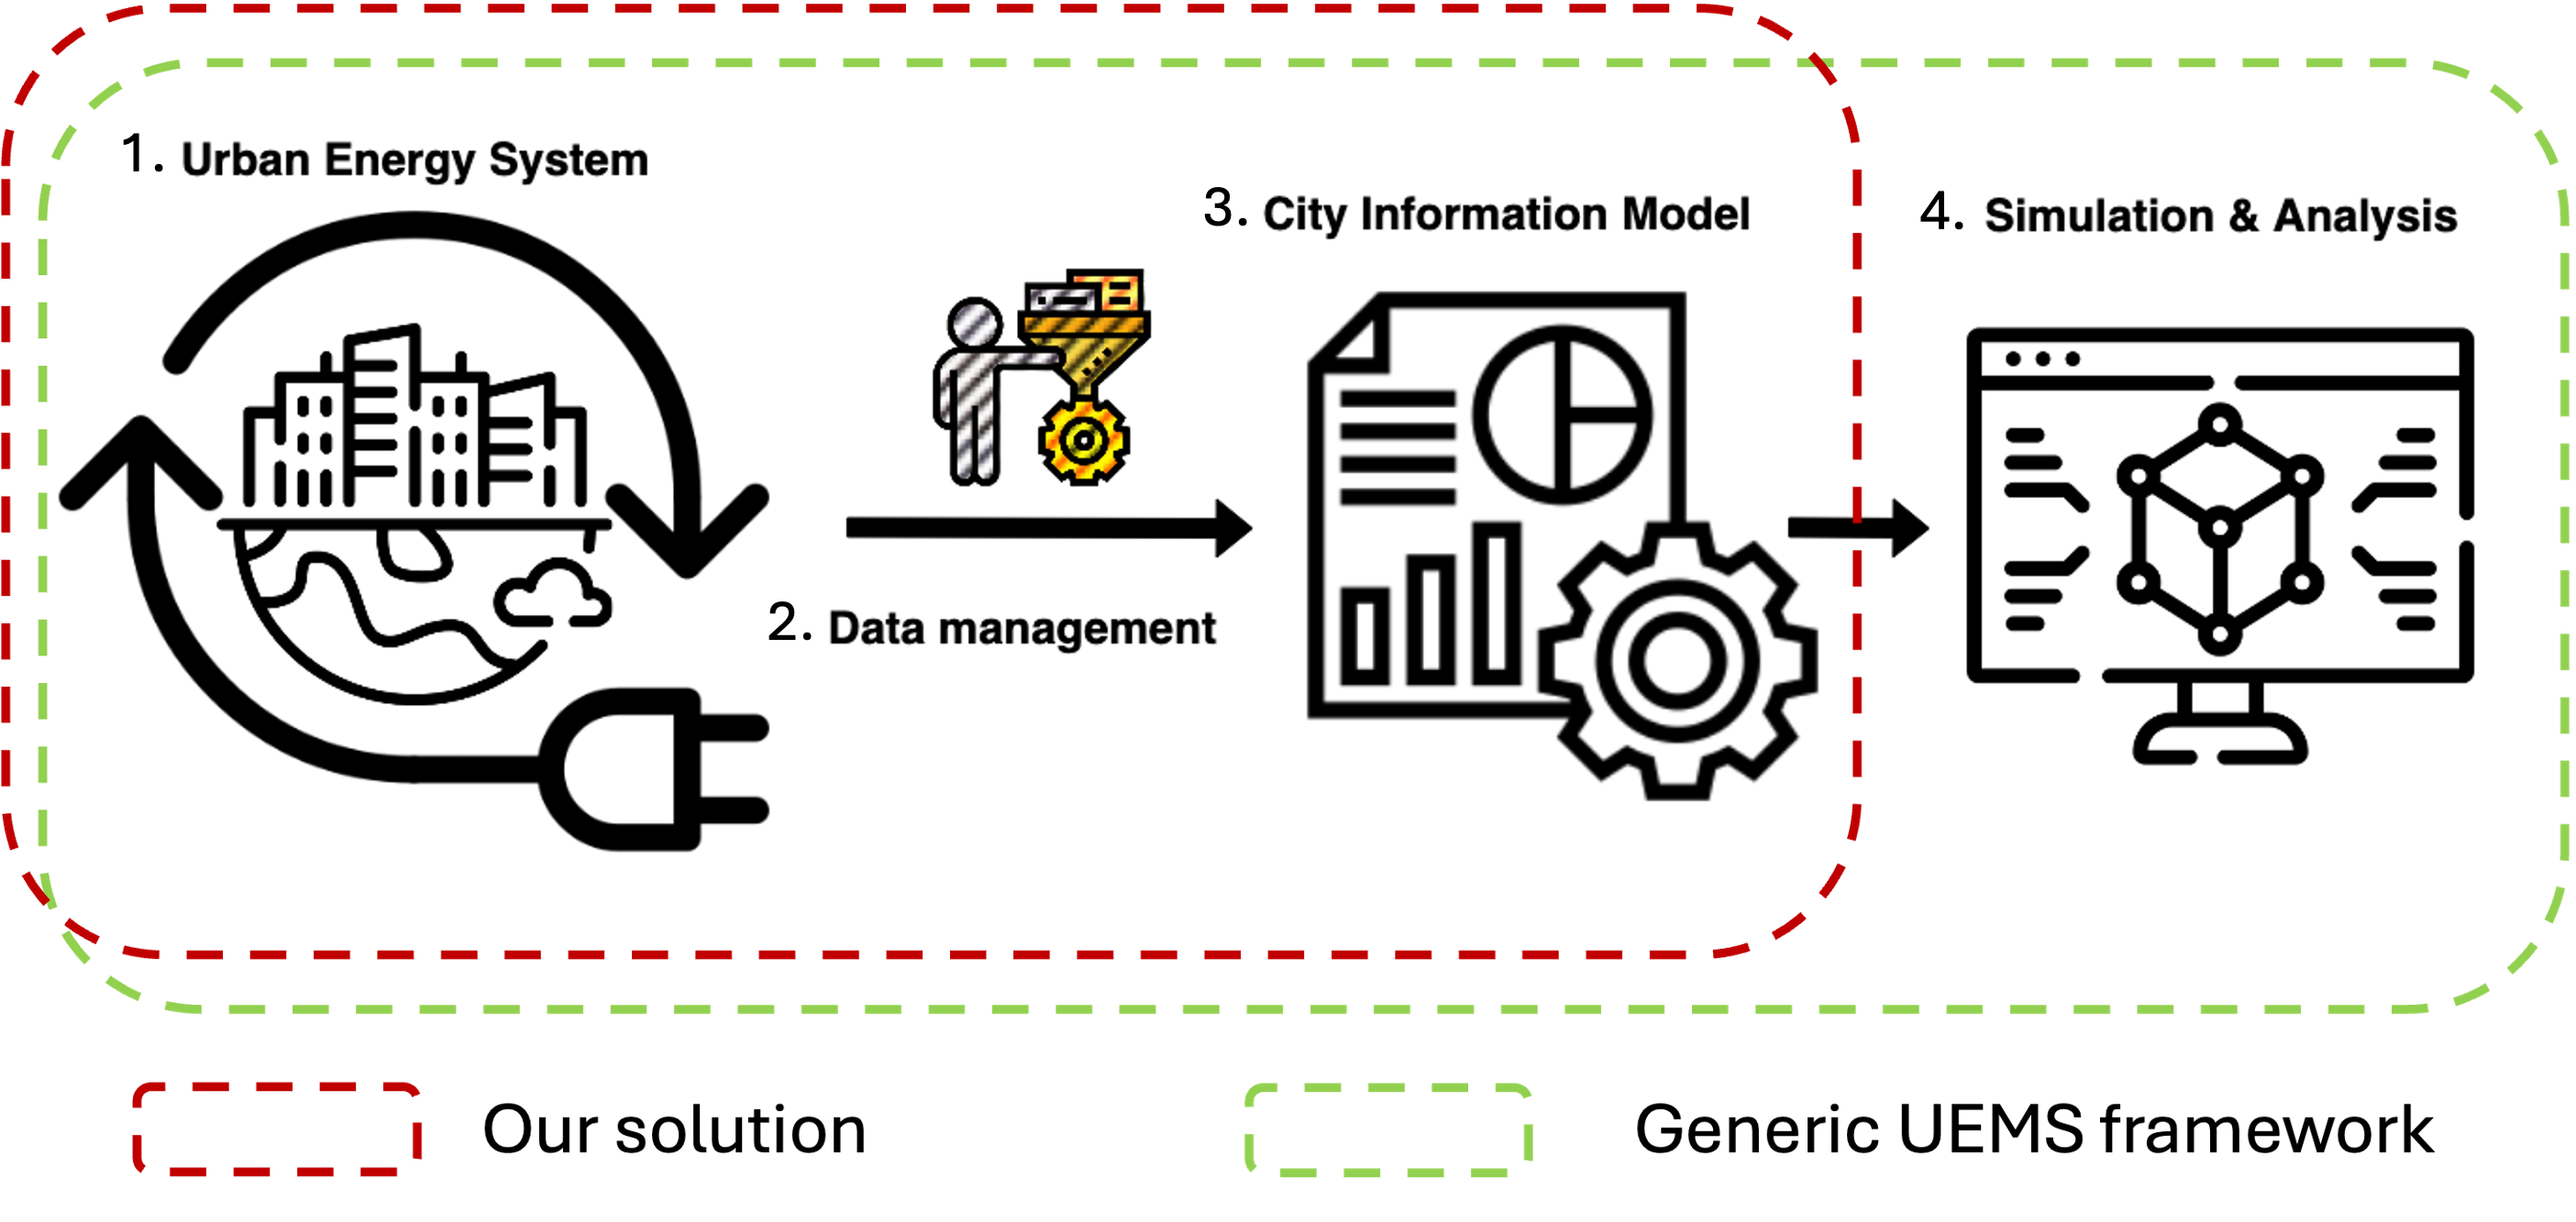
\includegraphics[width=0.95\textwidth,height=0.55\textheight,keepaspectratio]{figures/intro_workflow.png}
\end{column}
\end{columns}
\end{frame}

\begin{frame}{Research Problem: Three Interrelated Challenges}
\begin{columns}
\begin{column}{0.5\textwidth}
\textbf{1. Platform Challenge}
\begin{itemize}
    \item Need extensible framework for custom building property calculators
    \item Researchers shouldn't modify core infrastructure
\end{itemize}

\vspace{0.3cm}
\textbf{2. Data Challenge}
\begin{itemize}
    \item Large-scale datasets needed
    \item Manual annotation: \$0.50-1.00/sample
    \item Existing benchmarks lack spatial SQL coverage
\end{itemize}
\end{column}
\begin{column}{0.5\textwidth}
\textbf{3. Model Challenge}
\begin{itemize}
    \item General LLMs: 35-65\% accuracy baseline
    \item Multi-agent RAG vs Fine-tuning?
    \item Trade-offs: Privacy, Cost, CO$_2$, Quality
\end{itemize}

\vspace{0.3cm}
\begin{block}{Key Insight}
Intelligent built environments need both:
\begin{itemize}
    \item Information model generator (CIM Wizard)
    \item Natural language interface (CIM Assist)
\end{itemize}
\end{block}
\end{column}
\end{columns}
\end{frame}

\begin{frame}{Proposed Solution: Integrated Framework}
\centering
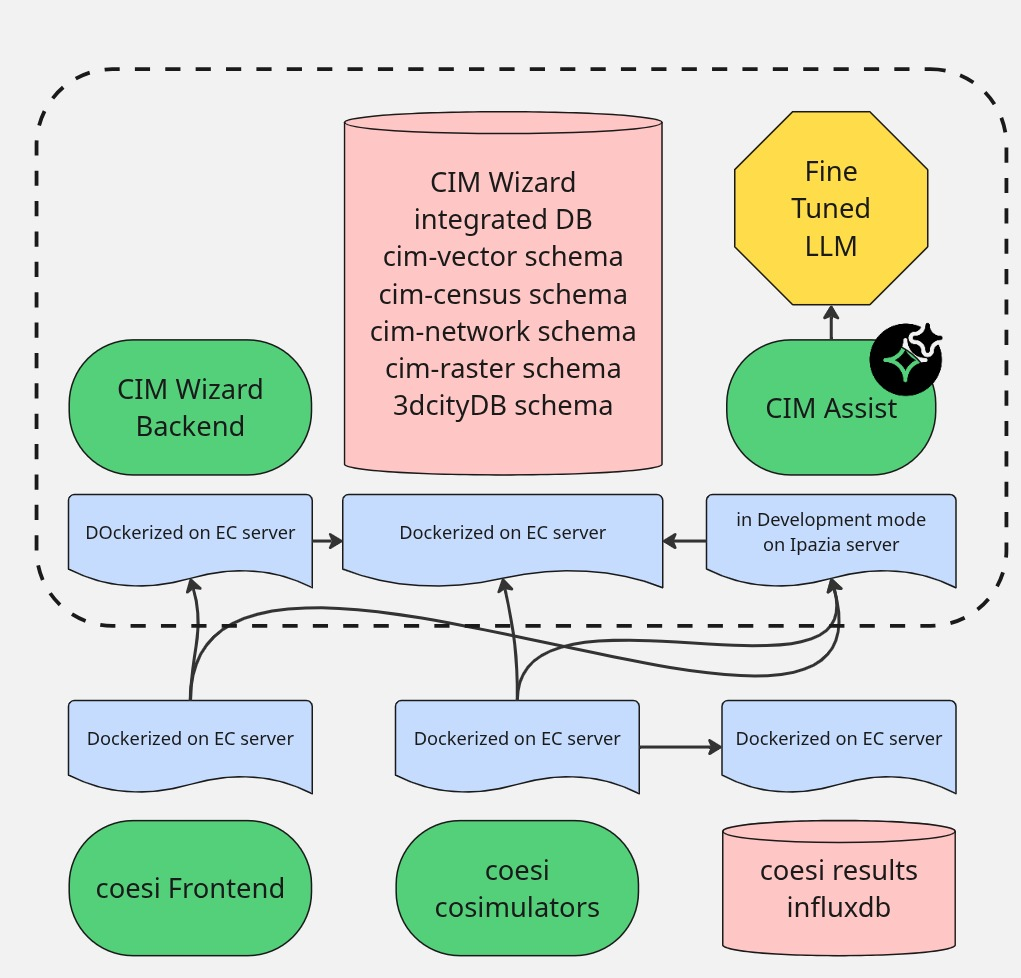
\includegraphics[width=0.9\textwidth,height=0.55\textheight,keepaspectratio]{figures/system-overview.jpg}
\vspace{0.2cm}
\textbf{Two Complementary Systems:}
\begin{columns}
\begin{column}{0.5\textwidth}
\textbf{CIM Wizard:}
\begin{itemize}
    \item Object-oriented platform
    \item 17 modular calculators
    \item Multi-schema PostGIS integration
\end{itemize}
\end{column}
\begin{column}{0.5\textwidth}
\textbf{CIM Assist:}
\begin{itemize}
    \item LLM-powered interface
    \item Dataset generation pipeline
    \item Fine-tuned models + Agent integration
\end{itemize}
\end{column}
\end{columns}
\end{frame}

%=============================================================================
% STATE OF THE ART + BACKGROUND (~1 min, 1 slide)
%=============================================================================

\section{Background \& State of the Art}

\begin{frame}{Research Gaps \& Key Technologies}
\begin{columns}
\begin{column}{0.5\textwidth}
\textbf{Research Gaps Identified:}
\begin{itemize}
    \item \textbf{No Text-to-Spatial-SQL benchmarks}\\
    {\small Spider/BIRD lack PostGIS coverage}
    \item \textbf{Platform limitations}\\
    {\small CityBES, UBEM.io lack extensibility}
    \item \textbf{No NL interfaces for urban DBs}
    \item \textbf{No validation-first methodology}
\end{itemize}

\vspace{0.1cm}
\textbf{Performance Gap:}\\
Human: $>$85\% | Best auto: $\sim$73\% (CHASE-SQL)
\end{column}
\begin{column}{0.5\textwidth}
\textbf{Key Technologies:}

\vspace{0.1cm}
\textbf{PostGIS}: Spatial database extension\\
{\small ST\_Intersects, ST\_Distance, ST\_Buffer...}

\vspace{0.1cm}
\textbf{LLMs}: Decoder-only transformers\\
{\small SQLCoder 7B pre-trained on BIRD}

\vspace{0.1cm}
\textbf{QLoRA}: Parameter-efficient fine-tuning\\
{\small 4-bit quantization $\rightarrow$ 14B on 24GB GPU}

\vspace{0.1cm}
\textbf{LangGraph}: Agent framework\\
{\small Iterative query refinement with tools}
\end{column}
\end{columns}
\end{frame}

%=============================================================================
% METHODOLOGY (~5 min, 5 slides) - MAIN FOCUS
%=============================================================================

\section{Methodology}

\begin{frame}{CIM Wizard: Calculator-Based Architecture}
\centering
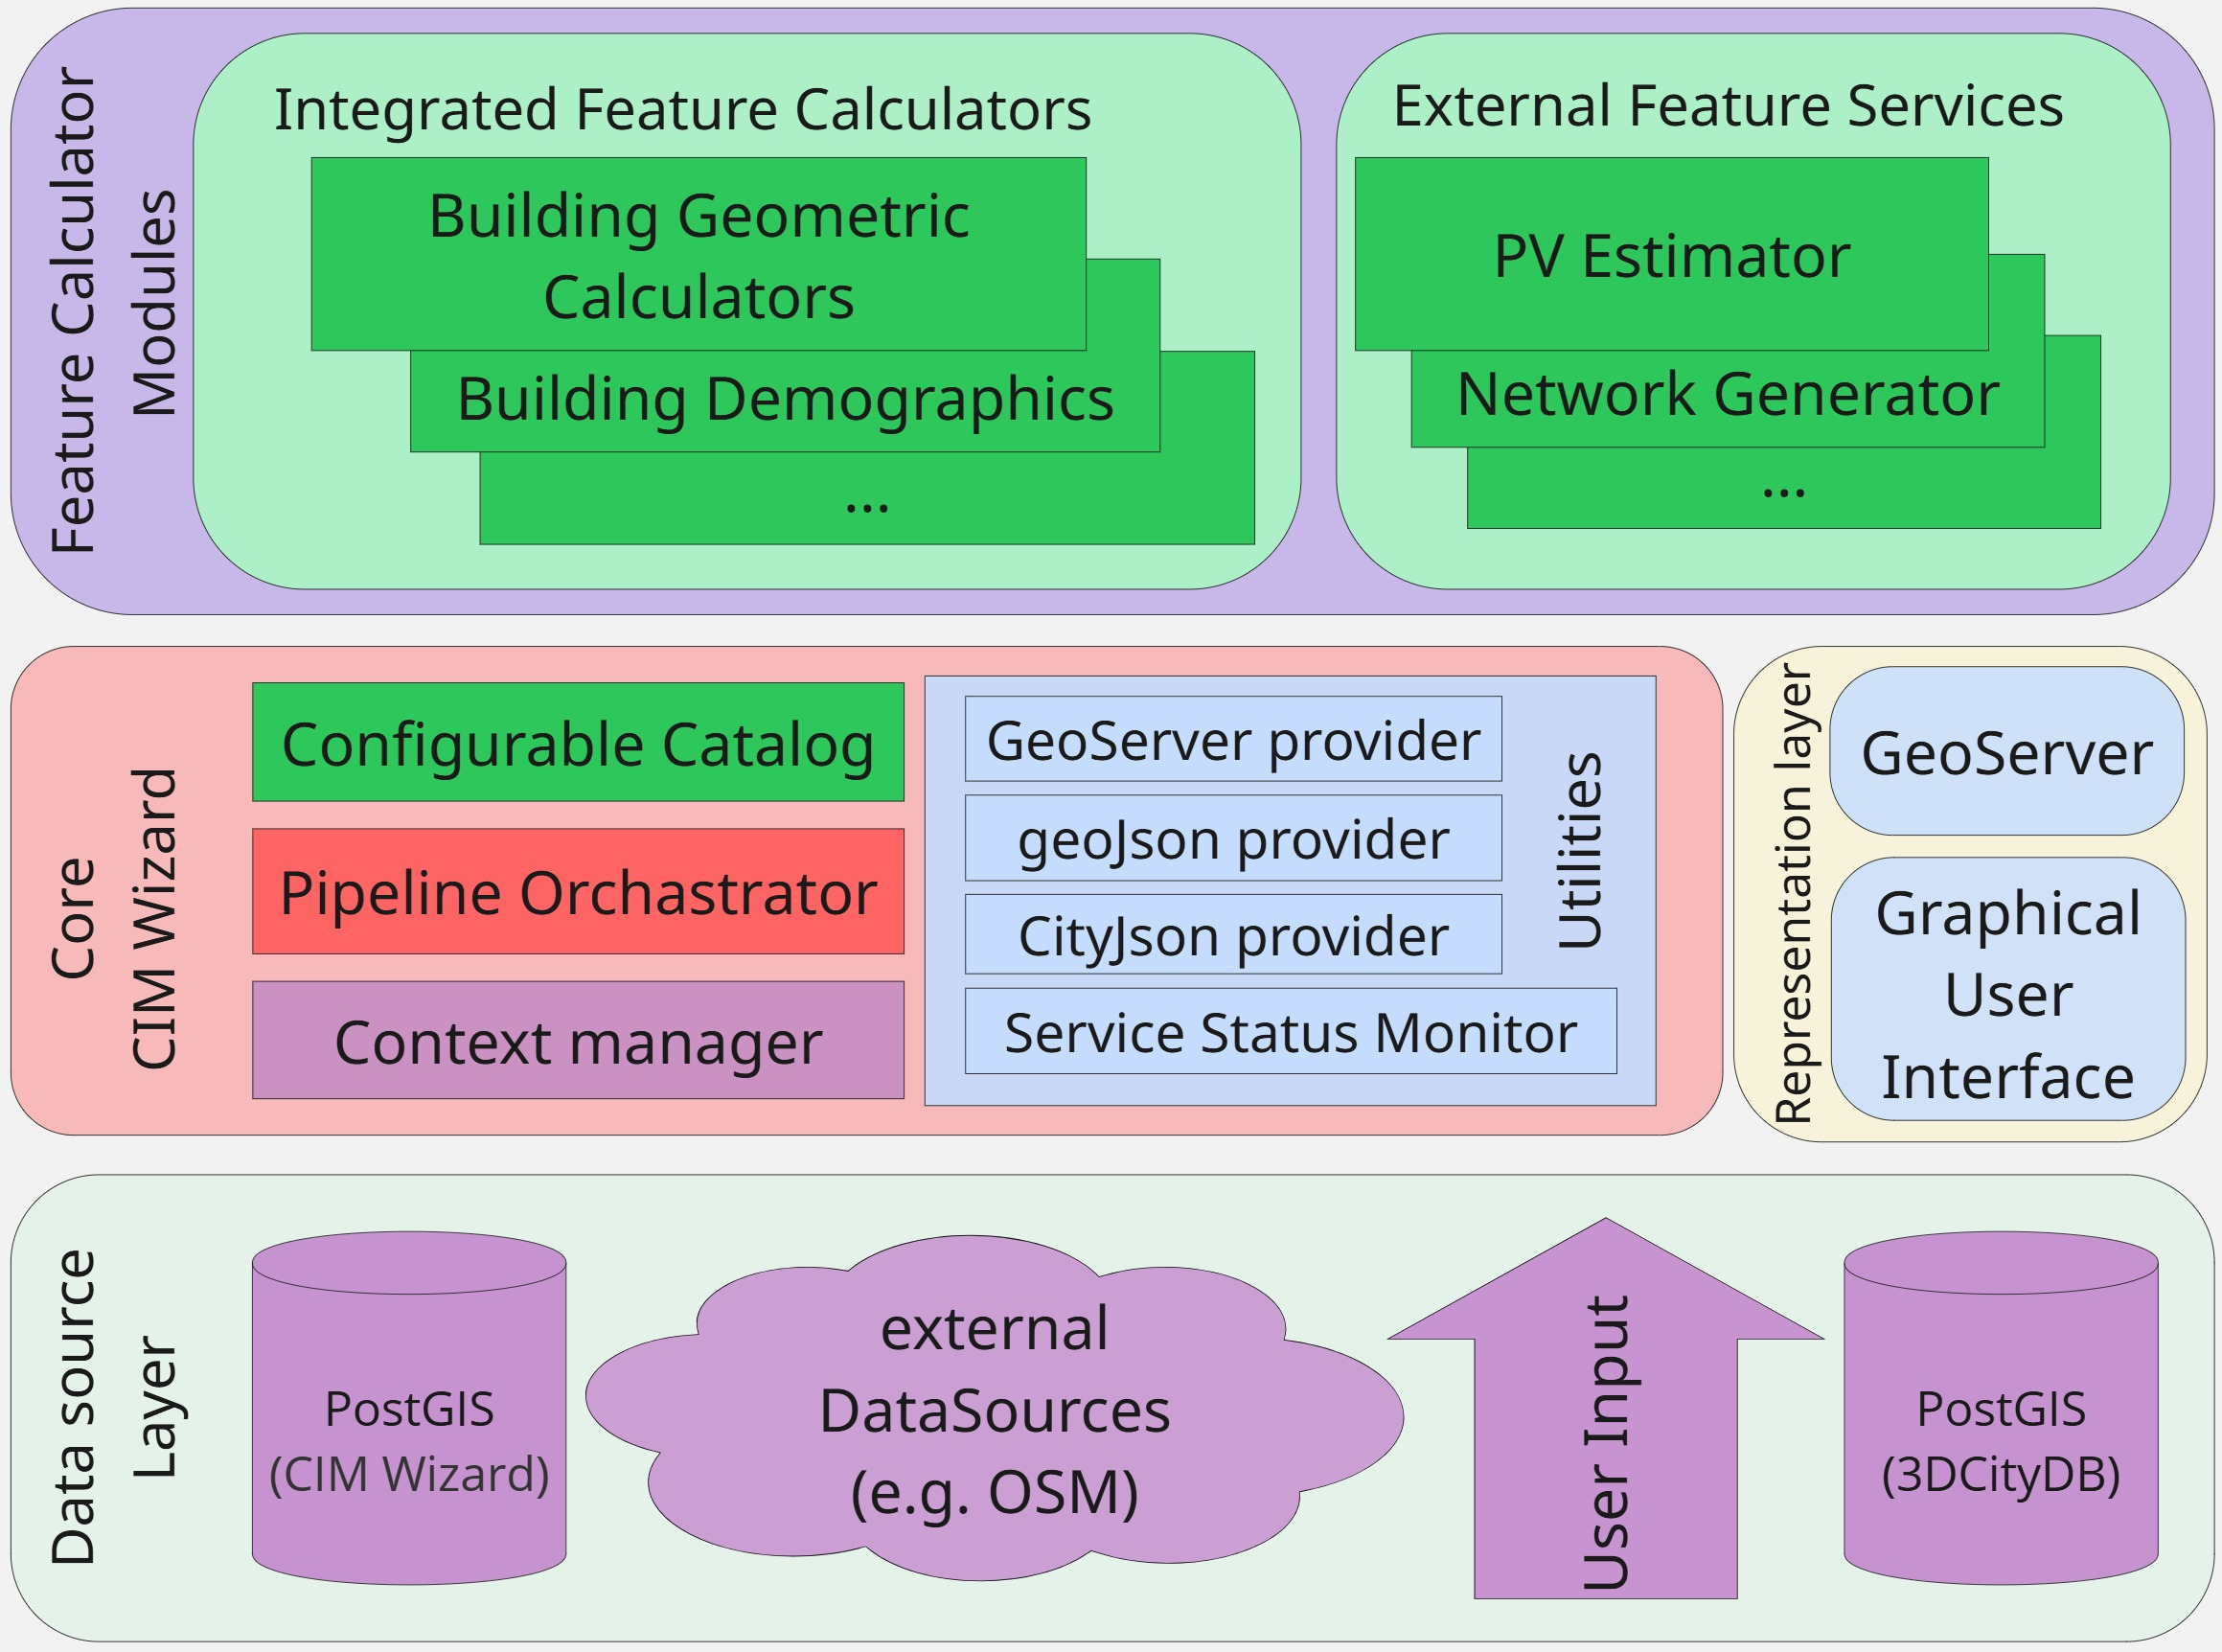
\includegraphics[width=0.7\textwidth,height=0.4\textheight,keepaspectratio]{figures/comet_arch.jpg}

\begin{columns}
\begin{column}{0.5\textwidth}
\textbf{Core Principles:}
\begin{itemize}
    \item \textbf{Extensibility}: Add calculators without core changes
    \item \textbf{Modularity}: Independent feature computation
    \item \textbf{Flexibility}: Multiple methods with fallbacks
\end{itemize}
\end{column}
\begin{column}{0.5\textwidth}
\textbf{Three PostGIS Schemas:}
\begin{itemize}
    \item \textbf{cim\_vector}: Building footprints, grid
    \item \textbf{cim\_census}: 100+ ISTAT attributes
    \item \textbf{cim\_raster}: DTM/DSM elevation
\end{itemize}
\end{column}
\end{columns}
\end{frame}

\begin{frame}{Calculator Example: Building Height with Fallbacks}
\centering
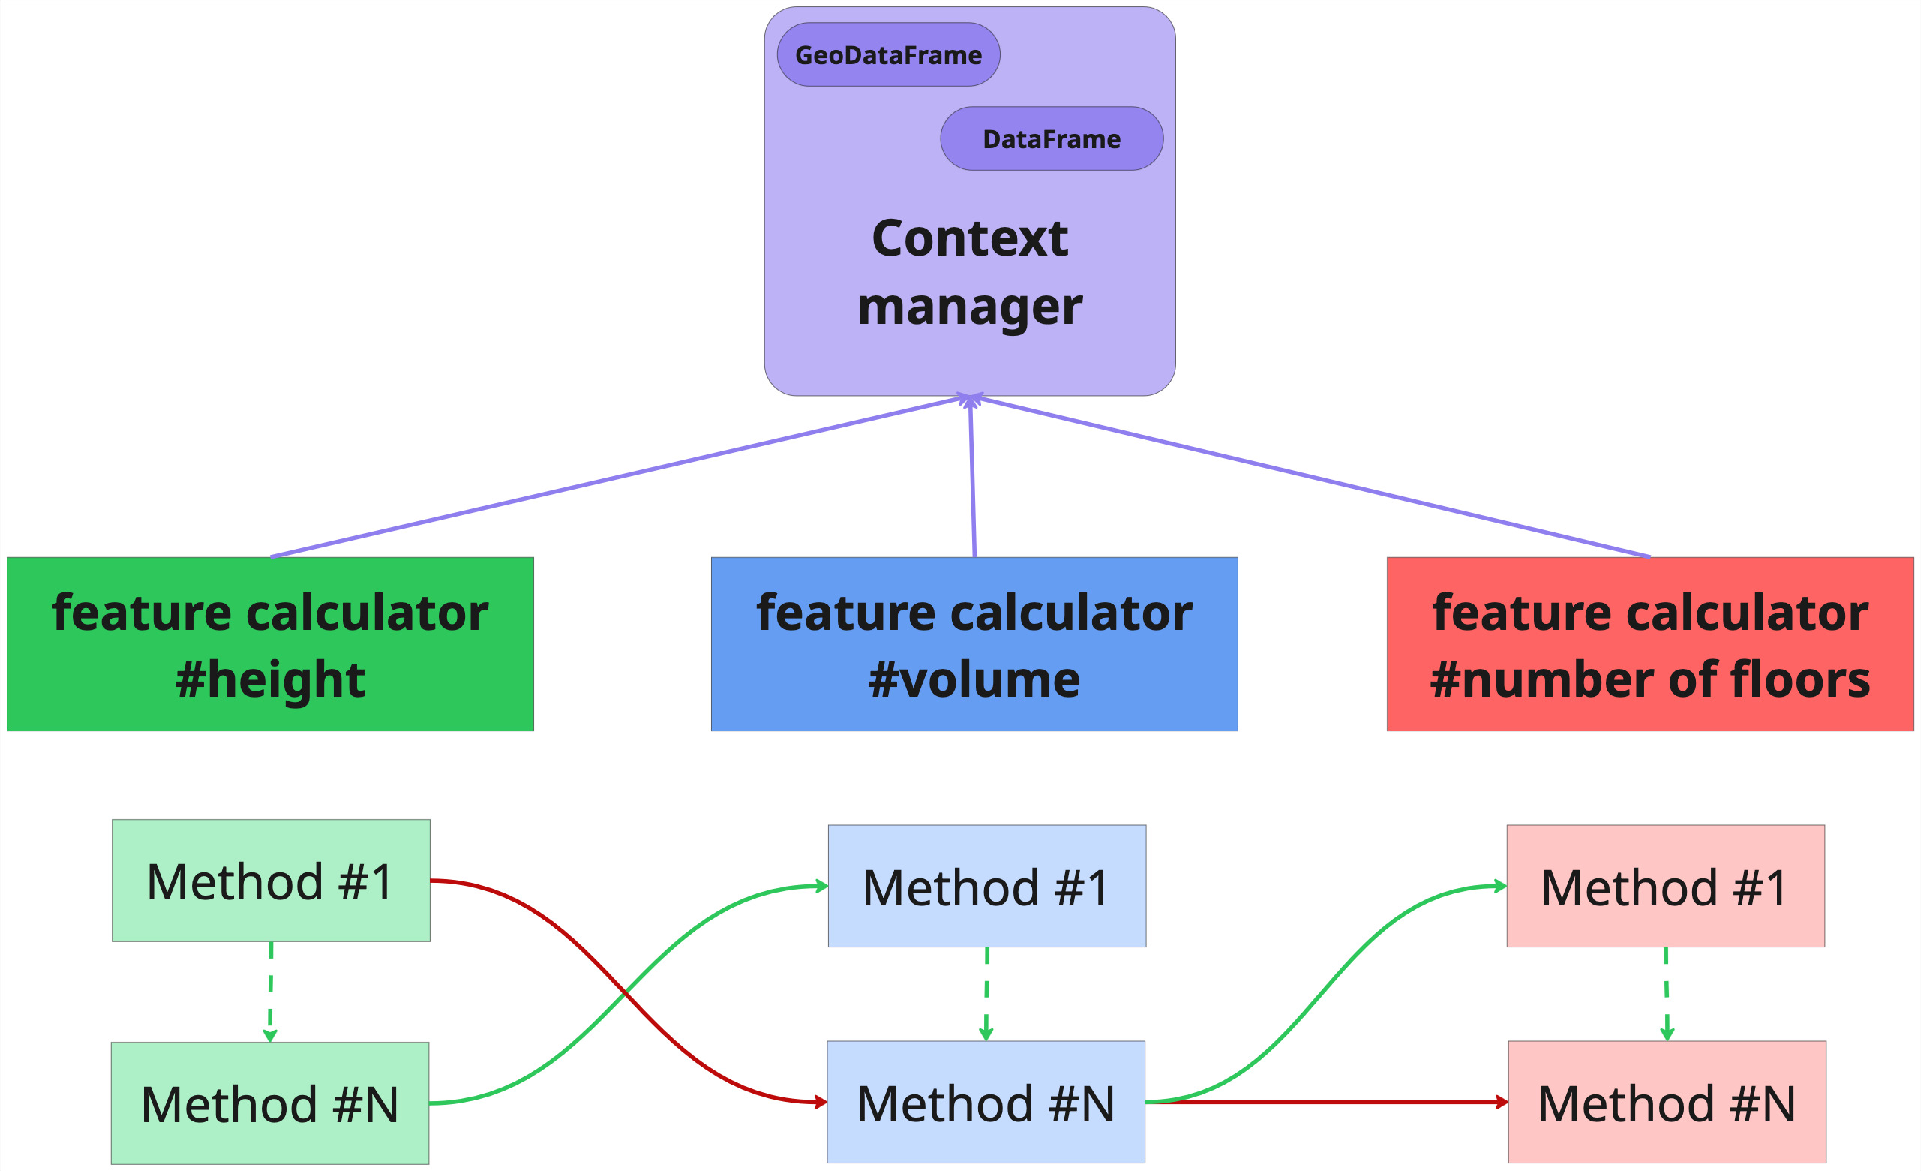
\includegraphics[width=0.65\textwidth,height=0.38\textheight,keepaspectratio]{figures/COMET-1.png}

\textbf{Three Fallback Methods:}
\begin{columns}
\begin{column}{0.33\textwidth}
\centering
\textbf{Method 1: Raster}\\
{\small DSM - DTM difference}\\
\textcolor{sintefgreen}{\textbf{Most accurate}}
\end{column}
\begin{column}{0.33\textwidth}
\centering
\textbf{Method 2: Census}\\
{\small Estimate from age}\\
\textcolor{sintefyellow}{\textbf{Fallback}}
\end{column}
\begin{column}{0.33\textwidth}
\centering
\textbf{Method 3: Default}\\
{\small 10m residential}\\
\textcolor{sintefred}{\textbf{Last resort}}
\end{column}
\end{columns}

\vspace{0.2cm}
\begin{block}{Key Innovation}
Automatic dependency resolution; researchers extend via class inheritance
\end{block}
\end{frame}

\begin{frame}{Dataset Generation: Two-Stage Pipeline}
\centering
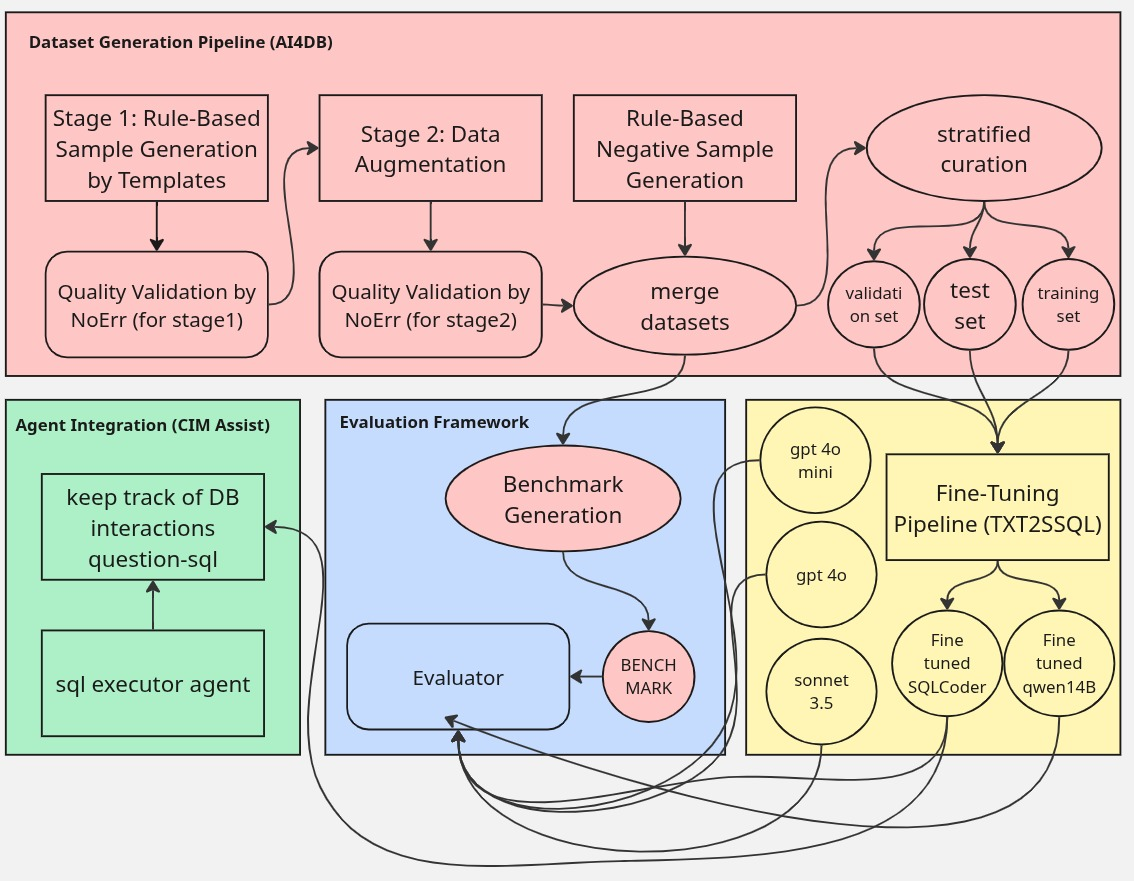
\includegraphics[width=0.8\textwidth,height=0.38\textheight,keepaspectratio]{figures/txt2ssql.jpg}

\begin{columns}
\begin{column}{0.5\textwidth}
\textbf{Stage 1: Rule-Based Templates}
\begin{itemize}
    \item 52 templates, 11 SQL types
    \item \textbf{10,800 samples}
    \item \textbf{98-100\% NoErr rate}
\end{itemize}
\end{column}
\begin{column}{0.5\textwidth}
\textbf{Stage 2: LLM Augmentation}
\begin{itemize}
    \item GPT-4o-mini, 5 strategies
    \item \textbf{50,000 samples}
    \item \textbf{97.34\% NoErr, \$50 total}
\end{itemize}
\end{column}
\end{columns}

\vspace{0.1cm}
\begin{block}{Validation-First Methodology}
Quality validated at each stage $\rightarrow$ \textbf{71.5\% retention} (vs. 10-30\% sequential)
\end{block}
\end{frame}

\begin{frame}{Fine-Tuning: QLoRA Configuration}
\begin{columns}
\begin{column}{0.55\textwidth}
\textbf{Training Setup:}
\begin{itemize}
    \item \textbf{Base Model}: SQLCoder 7B-2
    \item Pre-trained on Spider, BIRD benchmarks
    \item SQL-specific knowledge foundation
\end{itemize}

\vspace{0.3cm}
\textbf{QLoRA Configuration:}
\begin{itemize}
    \item 4-bit quantization (NF4)
    \item LoRA rank: 16, alpha: 32
    \item Target: attention + MLP layers
    \item \textbf{Only 0.12\% trainable params}
\end{itemize}

\vspace{0.3cm}
\textbf{Infrastructure:}
\begin{itemize}
    \item NVIDIA RTX 6000 24GB
    \item IPAZIA cluster (PoliTo)
    \item \textbf{Cost: \$0} (academic access)
\end{itemize}
\end{column}
\begin{column}{0.45\textwidth}
\centering
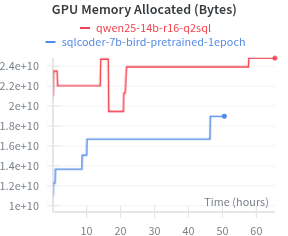
\includegraphics[width=0.95\textwidth,height=0.5\textheight,keepaspectratio]{figures/gpu_memory.png}
\vspace{0.2cm}
\begin{block}{Training Results}
\begin{itemize}
    \item \textbf{51 hours} training
    \item \textbf{18GB} memory usage
    \item \textbf{0.036} final loss
    \item No overfitting observed
\end{itemize}
\end{block}
\end{column}
\end{columns}
\end{frame}

\begin{frame}{Agent Integration for Evaluation}
\textbf{LangGraph-based Agent with Database Tools:}

\vspace{0.3cm}
\begin{columns}
\begin{column}{0.5\textwidth}
\textbf{Database Tools:}
\begin{itemize}
    \item \texttt{sql\_db\_list\_tables}: Discover tables
    \item \texttt{sql\_db\_schema}: Retrieve schemas
    \item \texttt{sql\_db\_query\_checker}: Validate SQL
    \item \texttt{sql\_db\_query}: Execute queries
\end{itemize}

\vspace{0.3cm}
\textbf{Self-Correction Loop:}
\begin{itemize}
    \item Up to 5 correction attempts
    \item Error feedback for refinement
    \item Automatic geometry detection
\end{itemize}
\end{column}
\begin{column}{0.5\textwidth}
\textbf{Evaluation Metrics:}
\begin{itemize}
    \item \textbf{NoErr}: Executable query rate
    \item \textbf{EX}: Execution accuracy (first-shot)
    \item \textbf{EA}: Eventual accuracy (with correction)
    \item \textbf{Deep EM}: Structural correctness
    \item \textbf{SC}: Semantic correctness
\end{itemize}

\vspace{0.3cm}
\begin{block}{Purpose}
Comprehensive evaluation through execution feedback reveals true model capability
\end{block}
\end{column}
\end{columns}
\end{frame}

%=============================================================================
% RESULTS (~5 min, 5 slides) - MAIN FOCUS
%=============================================================================

\section{Results}

\begin{frame}{CIM Wizard Validation: Turin Case Study}
\begin{columns}
\begin{column}{0.5\textwidth}
\centering
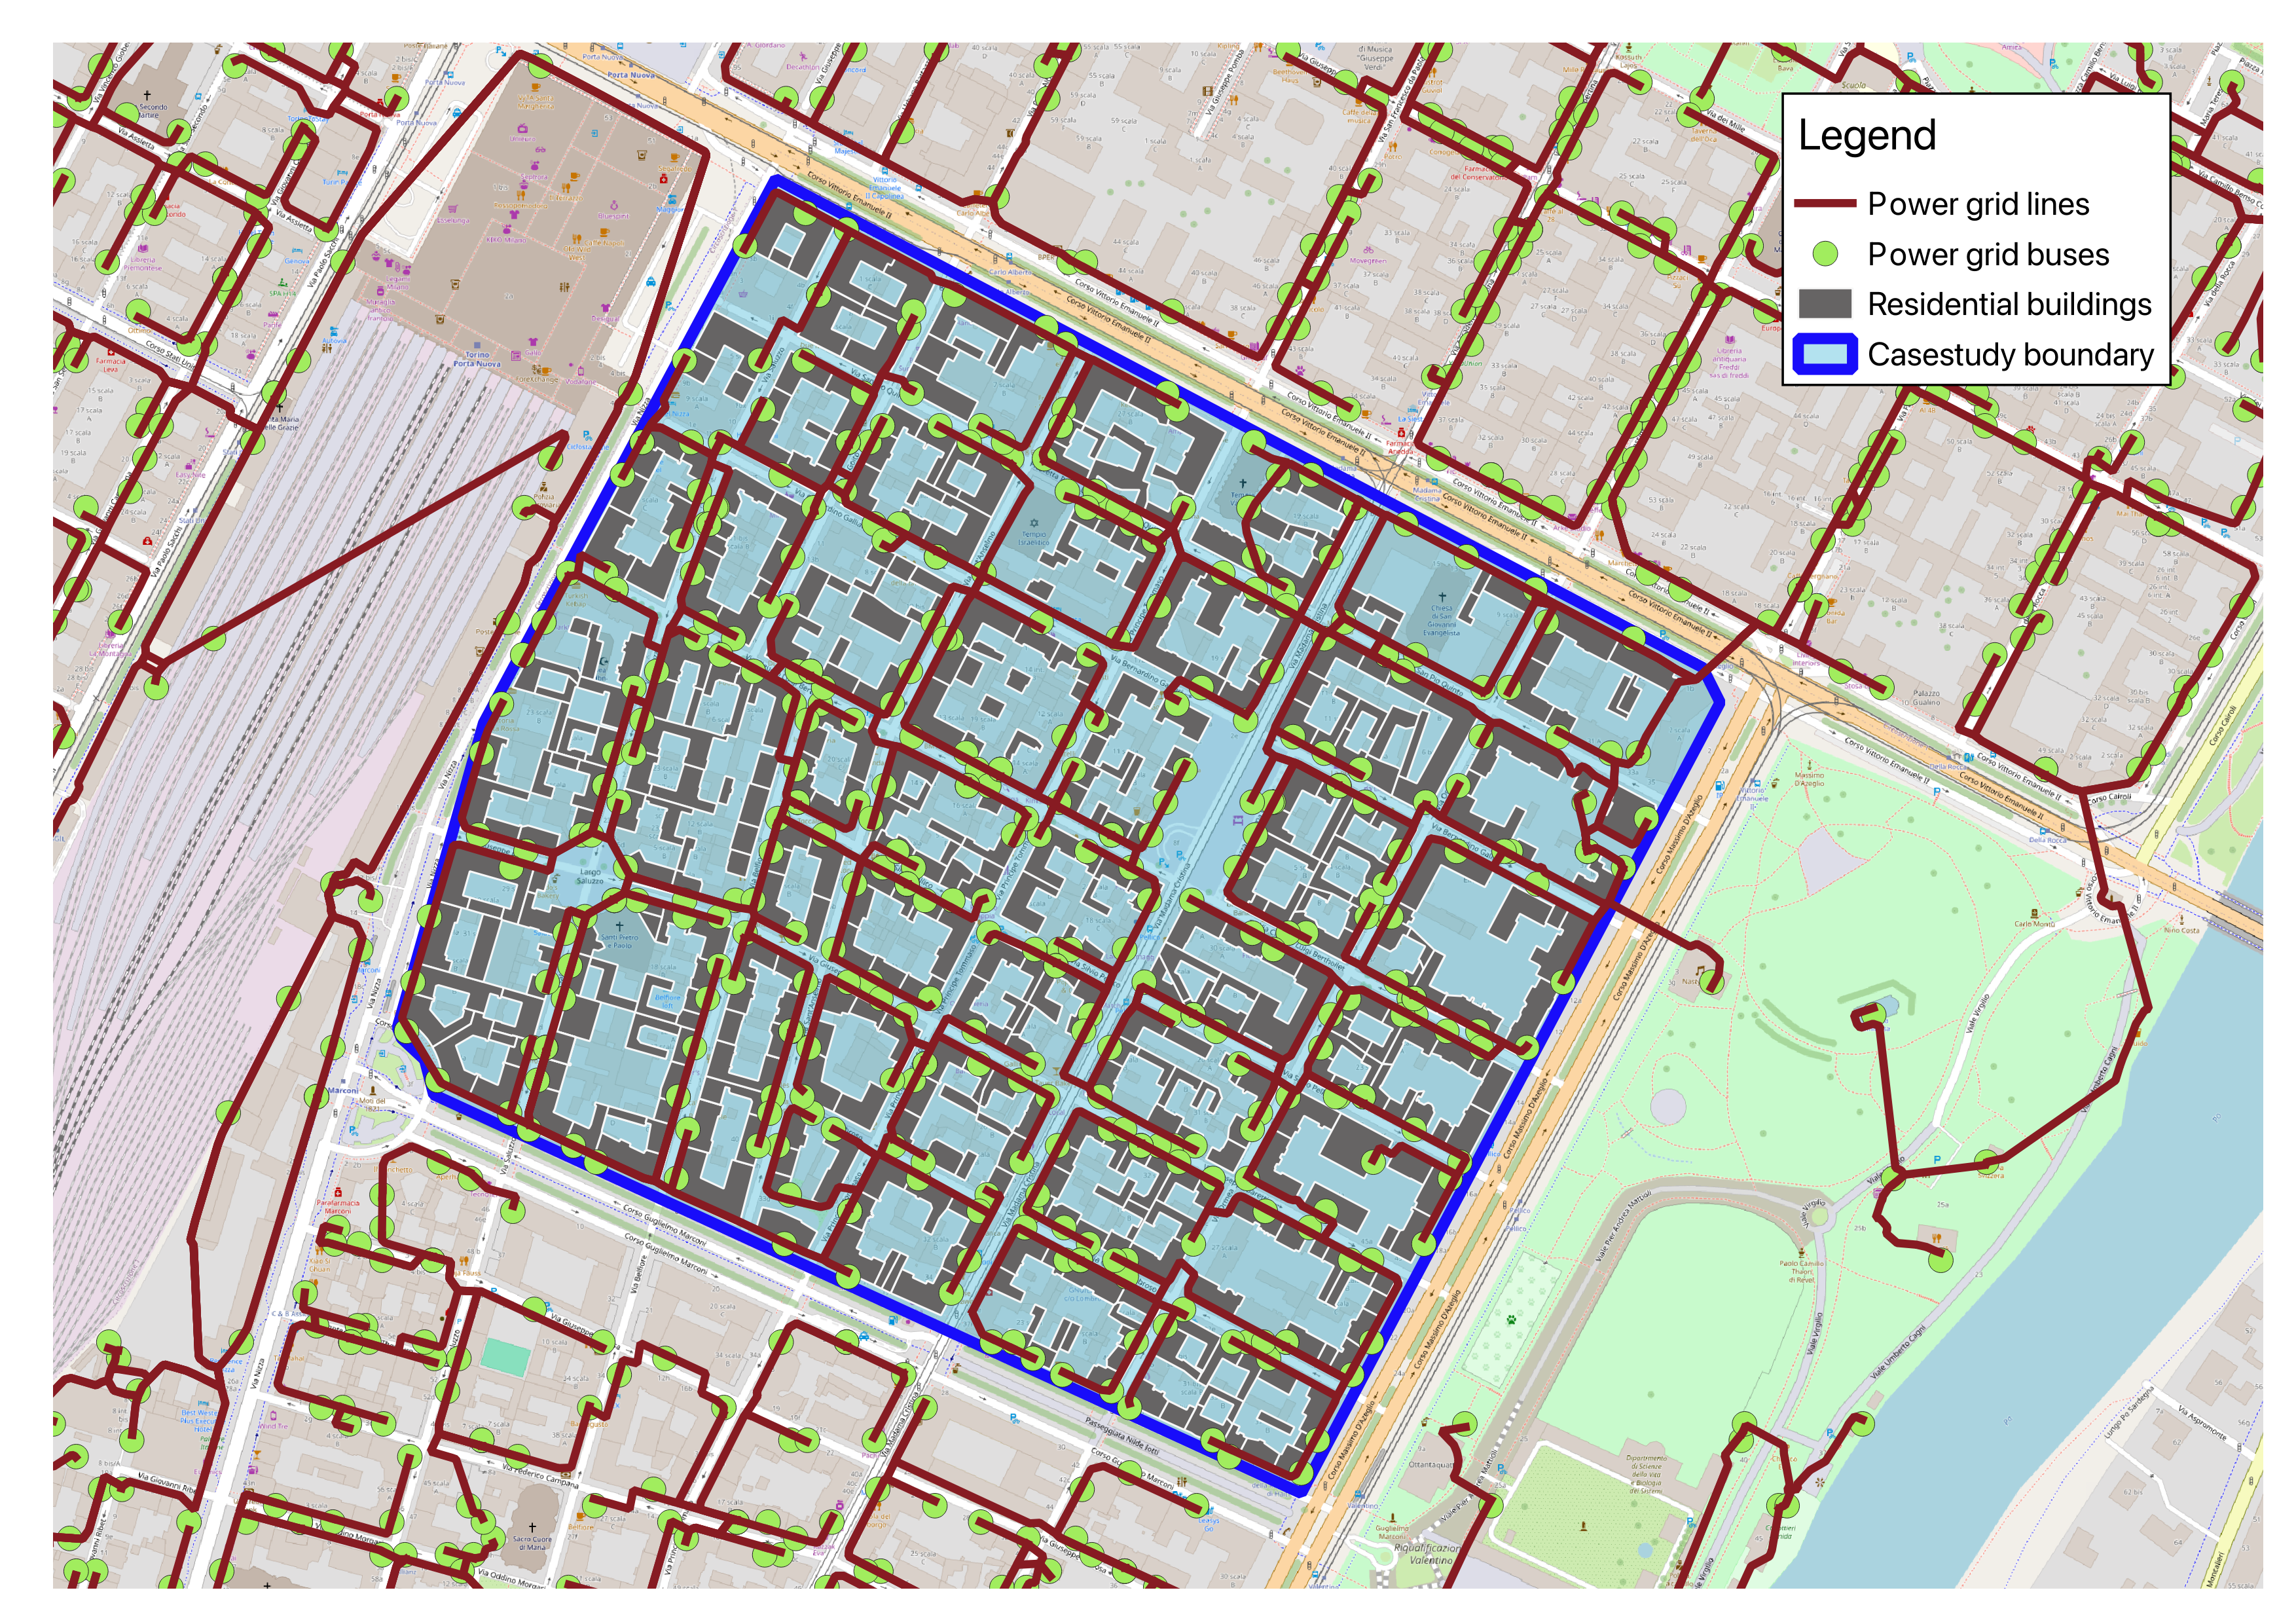
\includegraphics[width=0.95\textwidth,height=0.45\textheight,keepaspectratio]{figures/casestudy_finocchiaro.png}
\textbf{Sansalvario Neighborhood}
\begin{itemize}
    \item 552 buildings total
    \item 453 residential buildings
    \item Power grid network mapped
\end{itemize}
\end{column}
\begin{column}{0.5\textwidth}
\centering
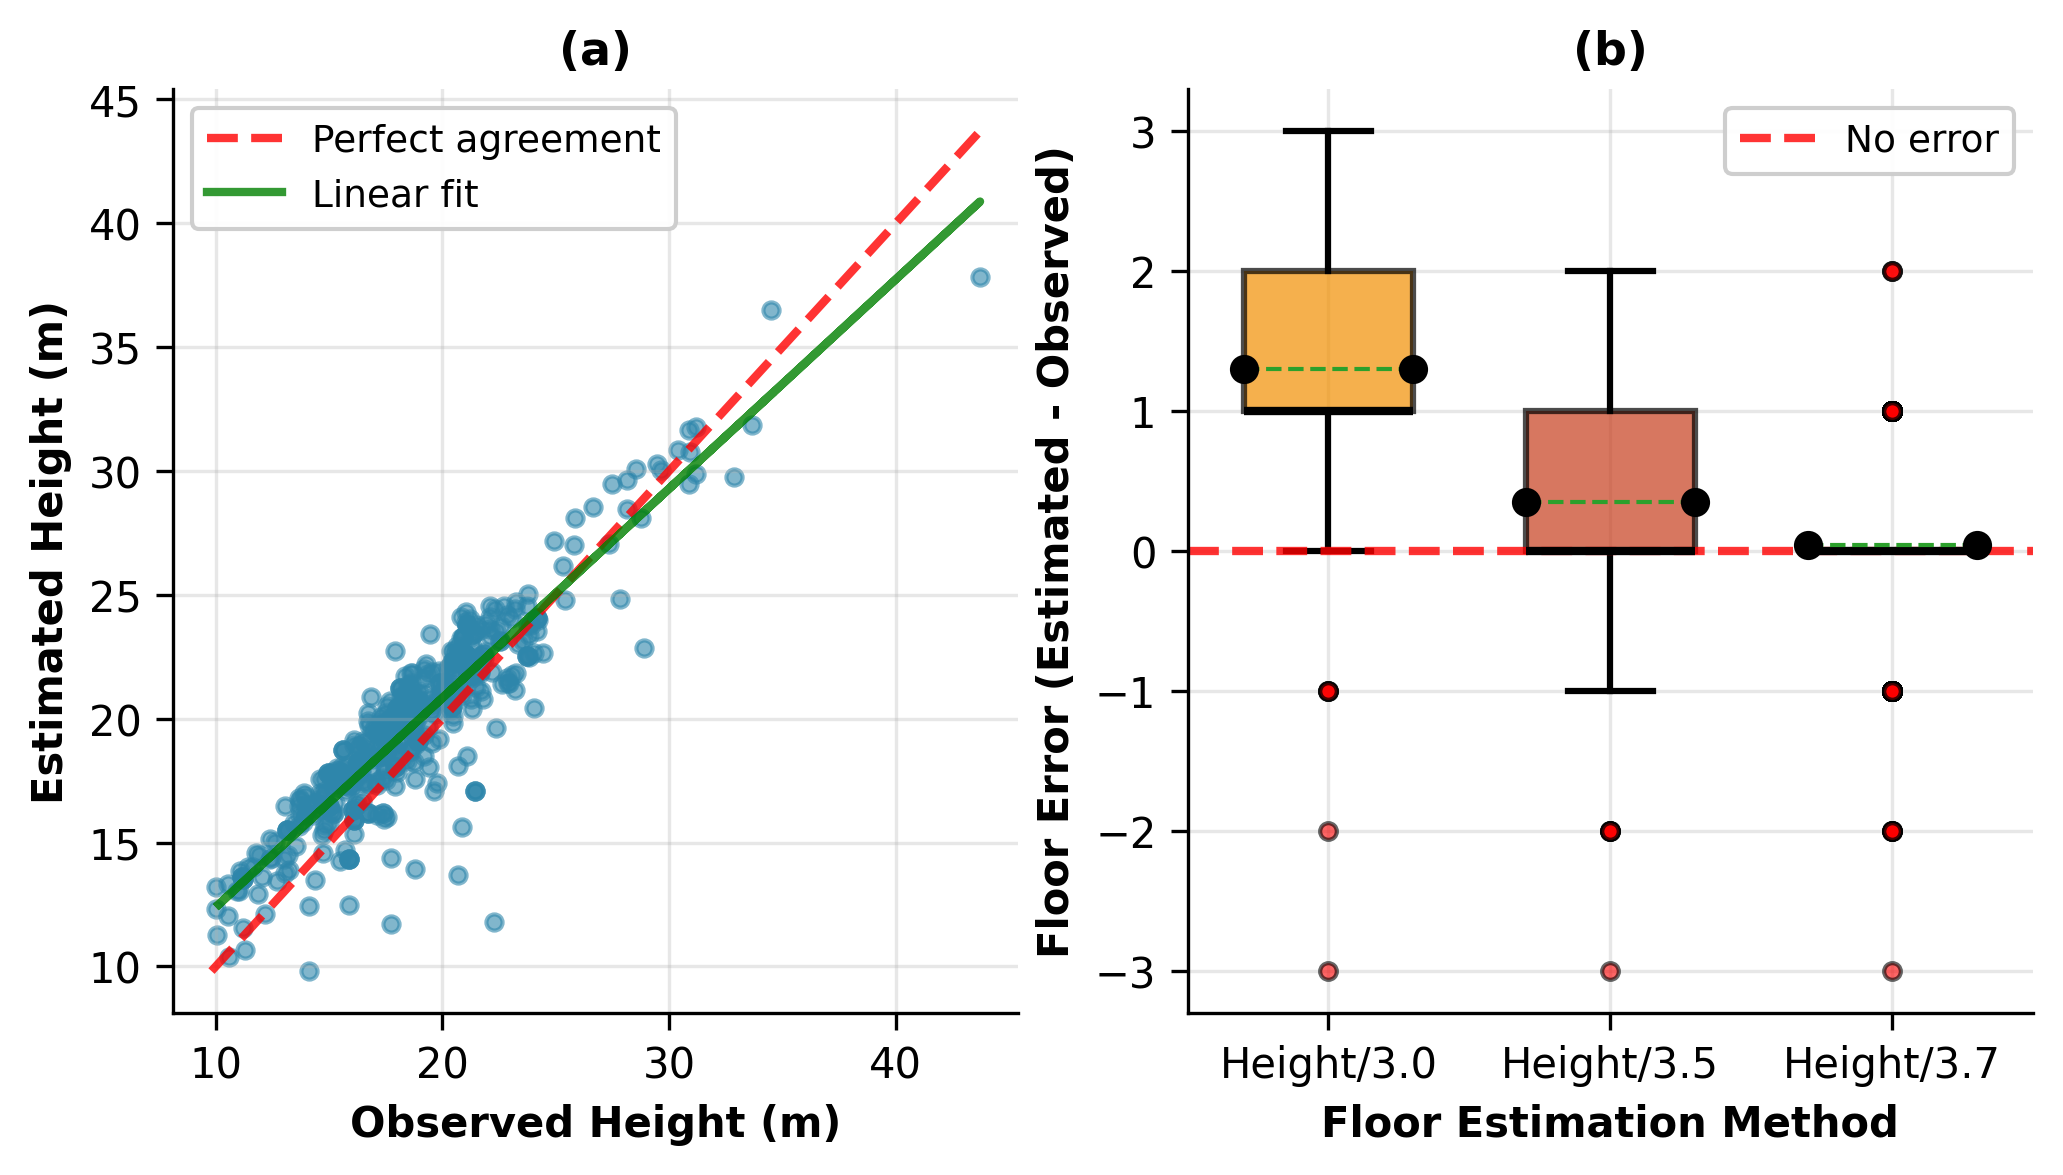
\includegraphics[width=0.95\textwidth,height=0.45\textheight,keepaspectratio]{figures/simplified_error_analysis.png}
\textbf{Validation Results:}
\begin{itemize}
    \item Height: Mean bias +1m
    \item Floors: 3.7m/floor optimal
    \item Construction periods match census
\end{itemize}
\end{column}
\end{columns}

\vspace{0.2cm}
\begin{block}{Performance}
Cross-schema queries execute in \textbf{<500ms} for 1000-5000 buildings
\end{block}
\end{frame}

\begin{frame}{The Key Result: 84.58\% Execution Accuracy}
\centering
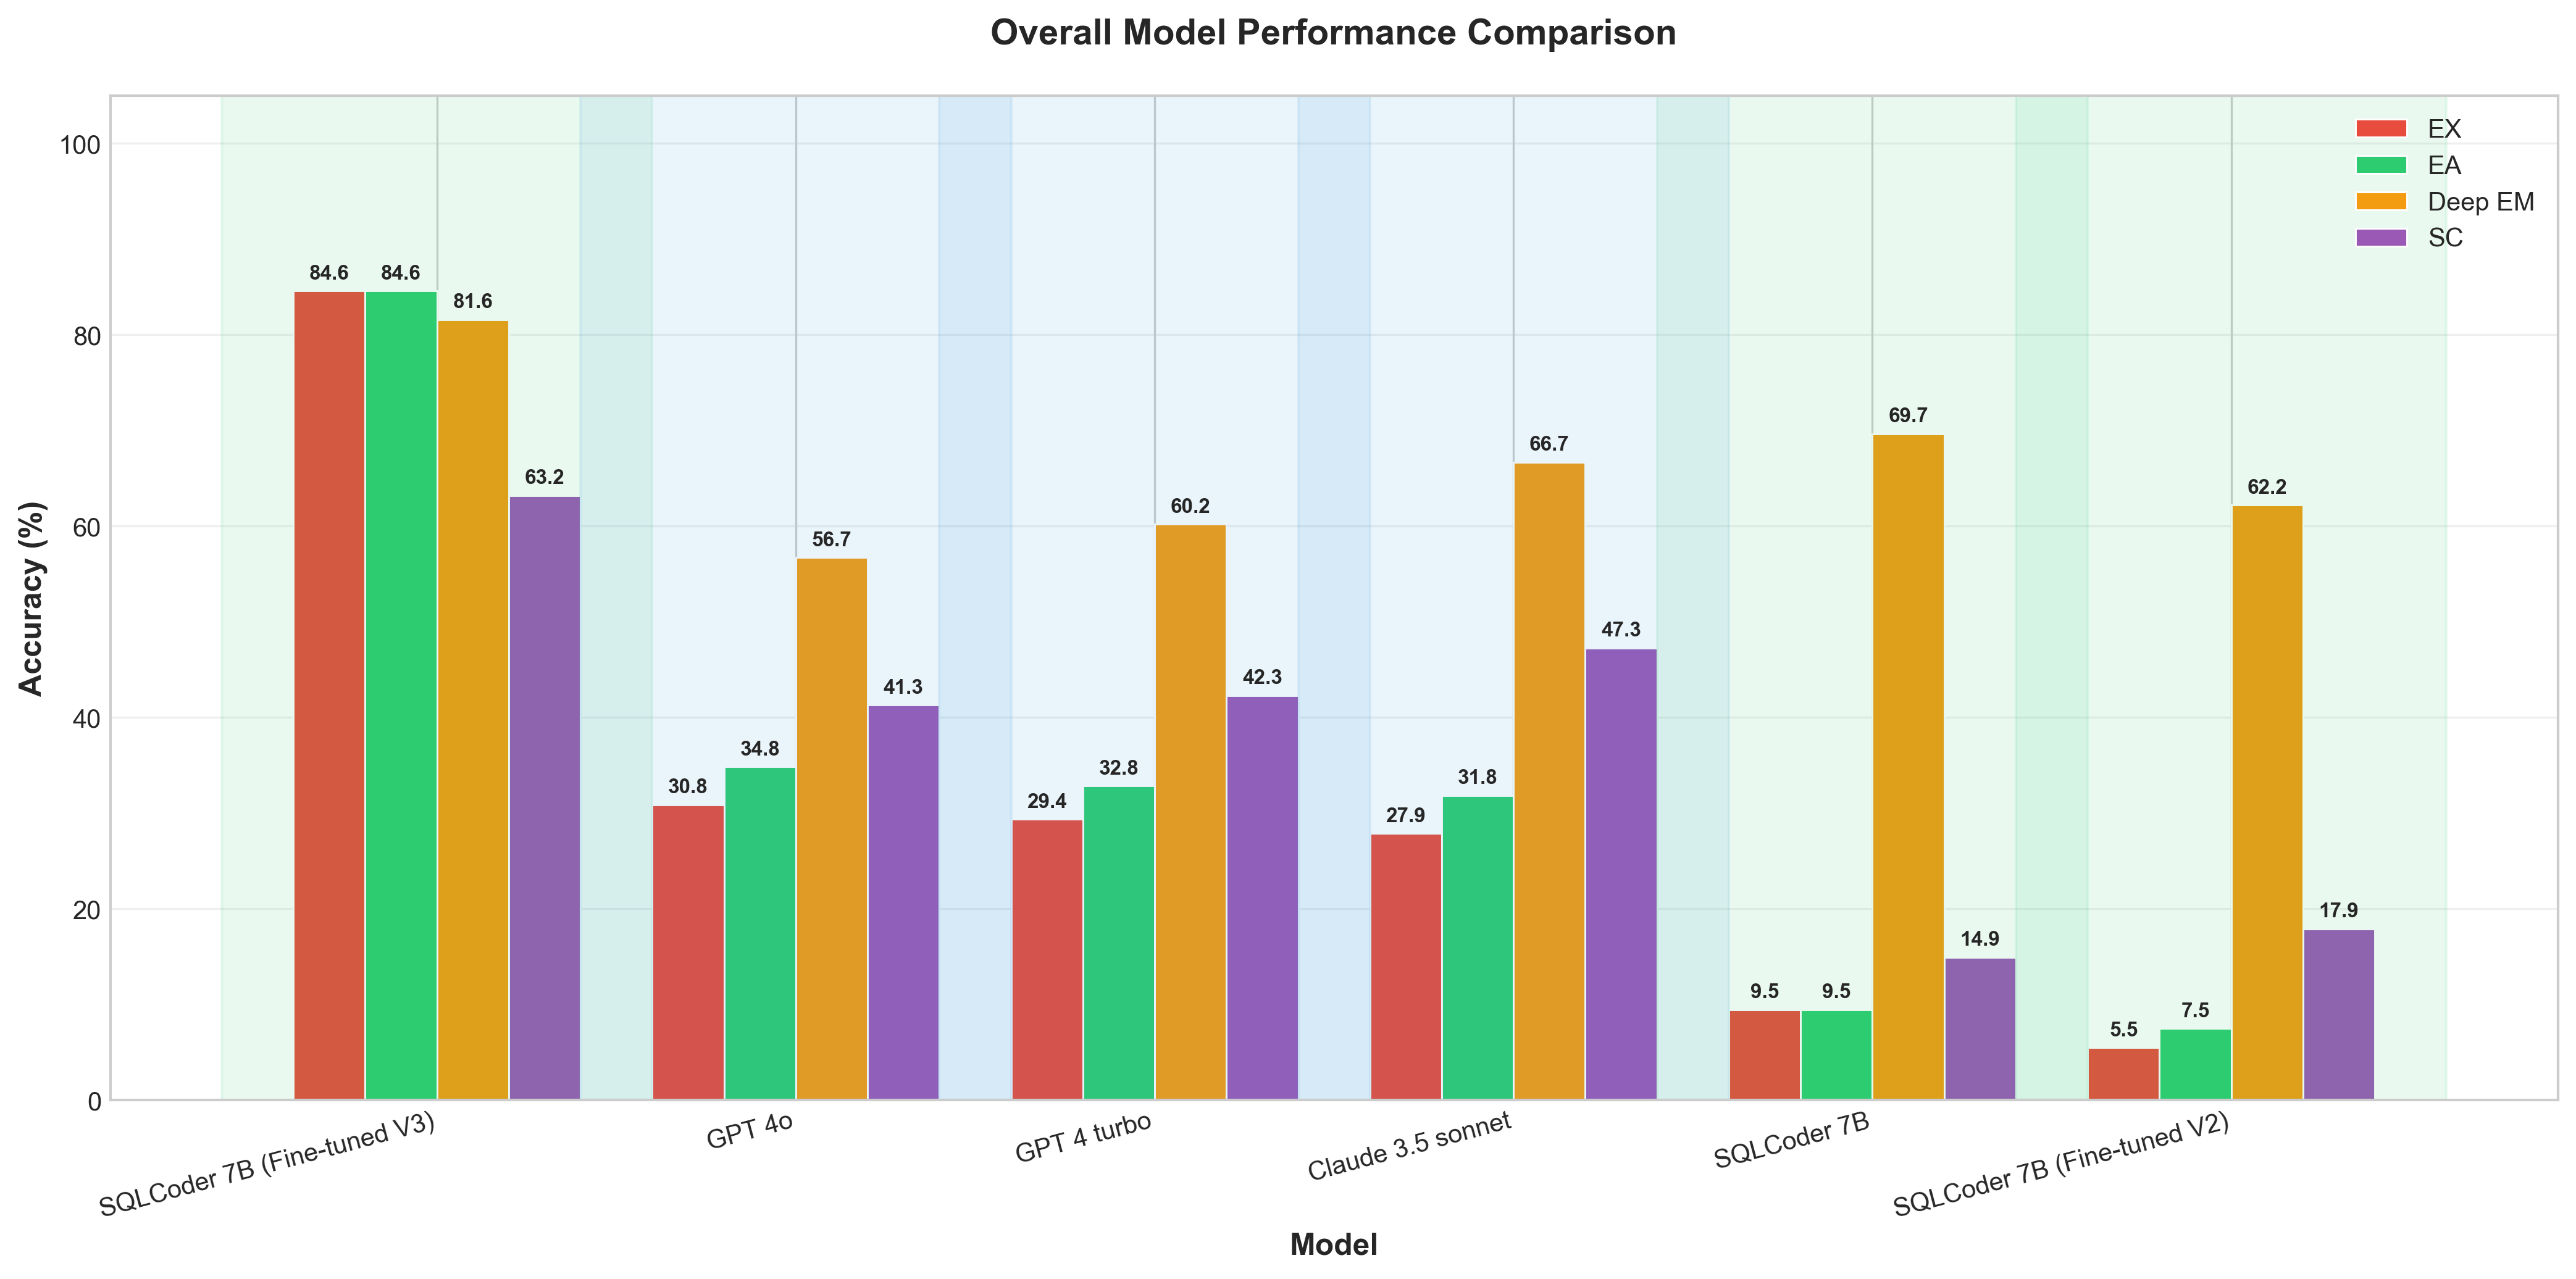
\includegraphics[width=0.95\textwidth,height=0.6\textheight,keepaspectratio]{figures/overall_comparison_bar.png}

\vspace{0.2cm}
\Large
\textbf{SQLCoder 7B (Fine-tuned): 84.58\% EX}\\
\normalsize
$\rightarrow$ \textcolor{sintefgreen}{\textbf{+54 percentage points}} above GPT-4o (30.85\%)

\vspace{0.2cm}
\begin{block}{Key Insight}
\textbf{Domain specialization beats model scale}: 7B fine-tuned > 100B+ general-purpose
\end{block}
\end{frame}

\begin{frame}{Performance by Task Type \& Complexity}
\begin{columns}
\begin{column}{0.55\textwidth}
\centering
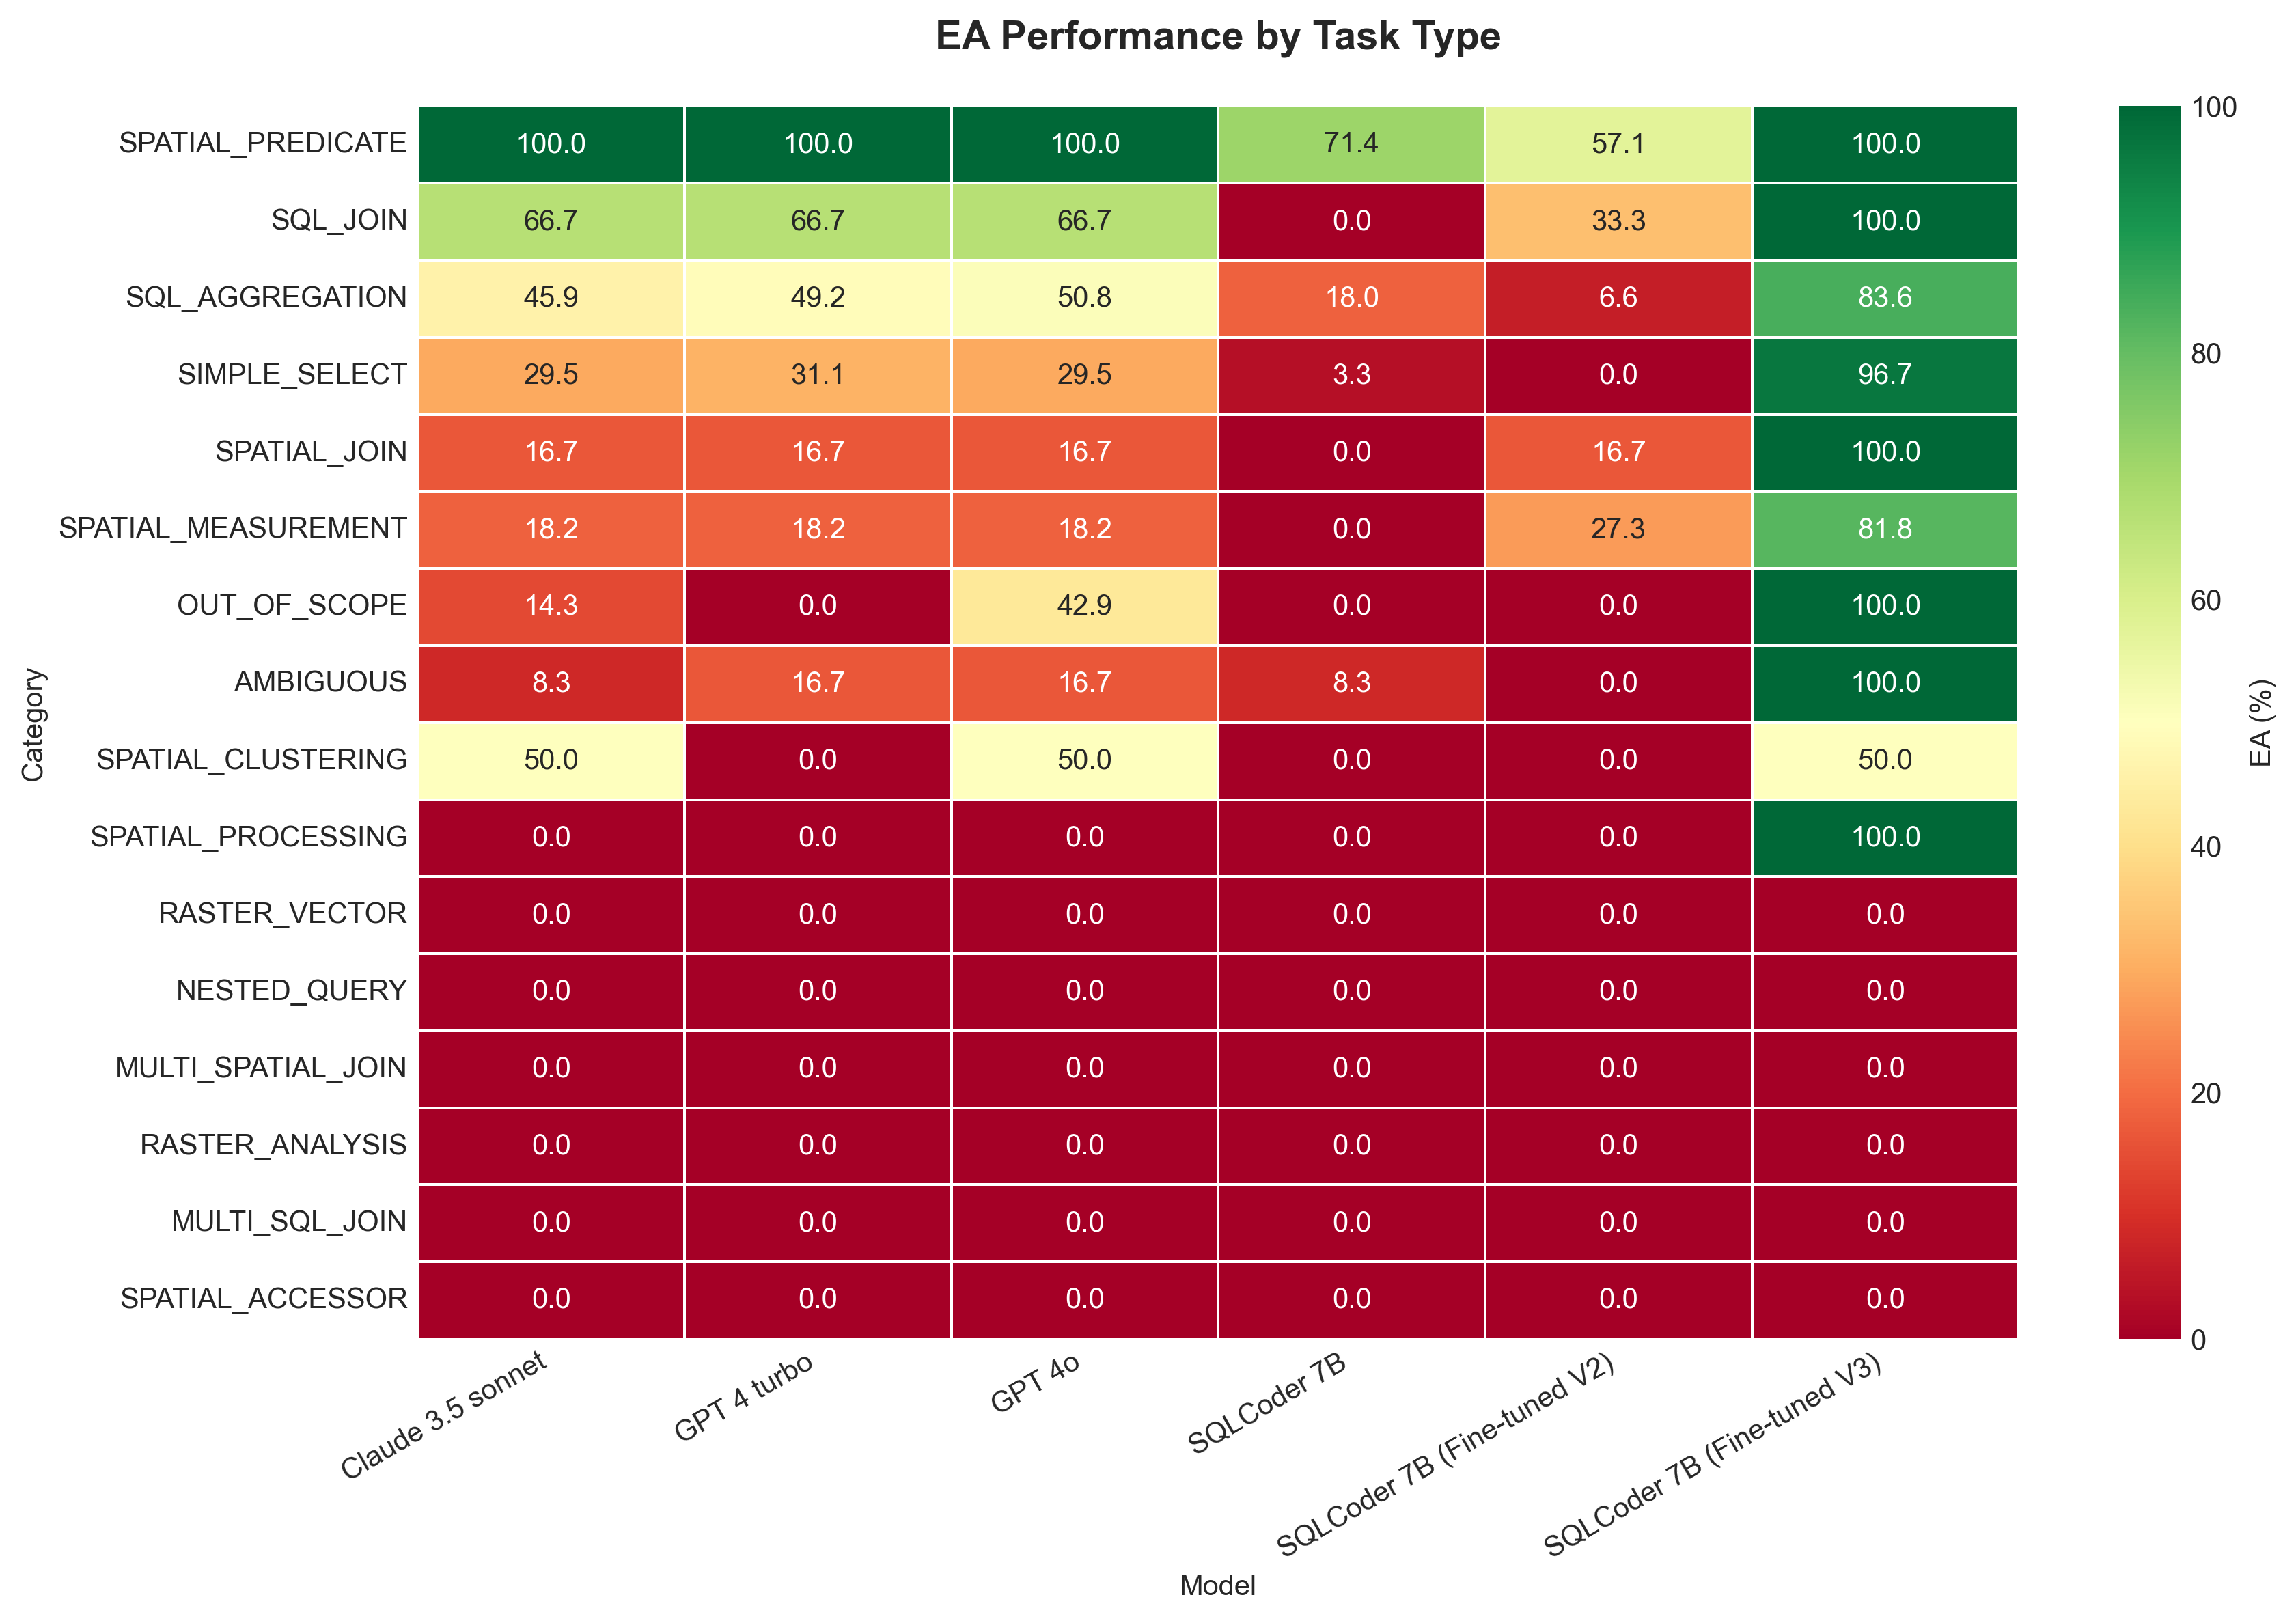
\includegraphics[width=0.95\textwidth,height=0.55\textheight,keepaspectratio]{figures/heatmap_task_type.png}
\end{column}
\begin{column}{0.45\textwidth}
\textbf{Task Type Performance:}
\begin{itemize}
    \item SIMPLE\_SELECT: 96.72\%
    \item SPATIAL\_JOIN: 88.89\%
    \item SPATIAL\_PREDICATE: \textbf{100\%}
    \item Multi-schema complex: 72.41\%
\end{itemize}

\vspace{0.3cm}
\textbf{Complexity Degradation:}
\begin{itemize}
    \item SQLCoder: -16pp (easy$\rightarrow$hard)
    \item GPT-4o: -27pp (45\%$\rightarrow$18\%)
\end{itemize}

\vspace{0.2cm}
\textcolor{sintefgreen}{\textbf{SQLCoder maintains robust performance even on complex multi-schema queries}}
\end{column}
\end{columns}
\end{frame}

\begin{frame}{Self-Correction Analysis: First-Shot Quality}
\begin{columns}
\begin{column}{0.55\textwidth}
\centering
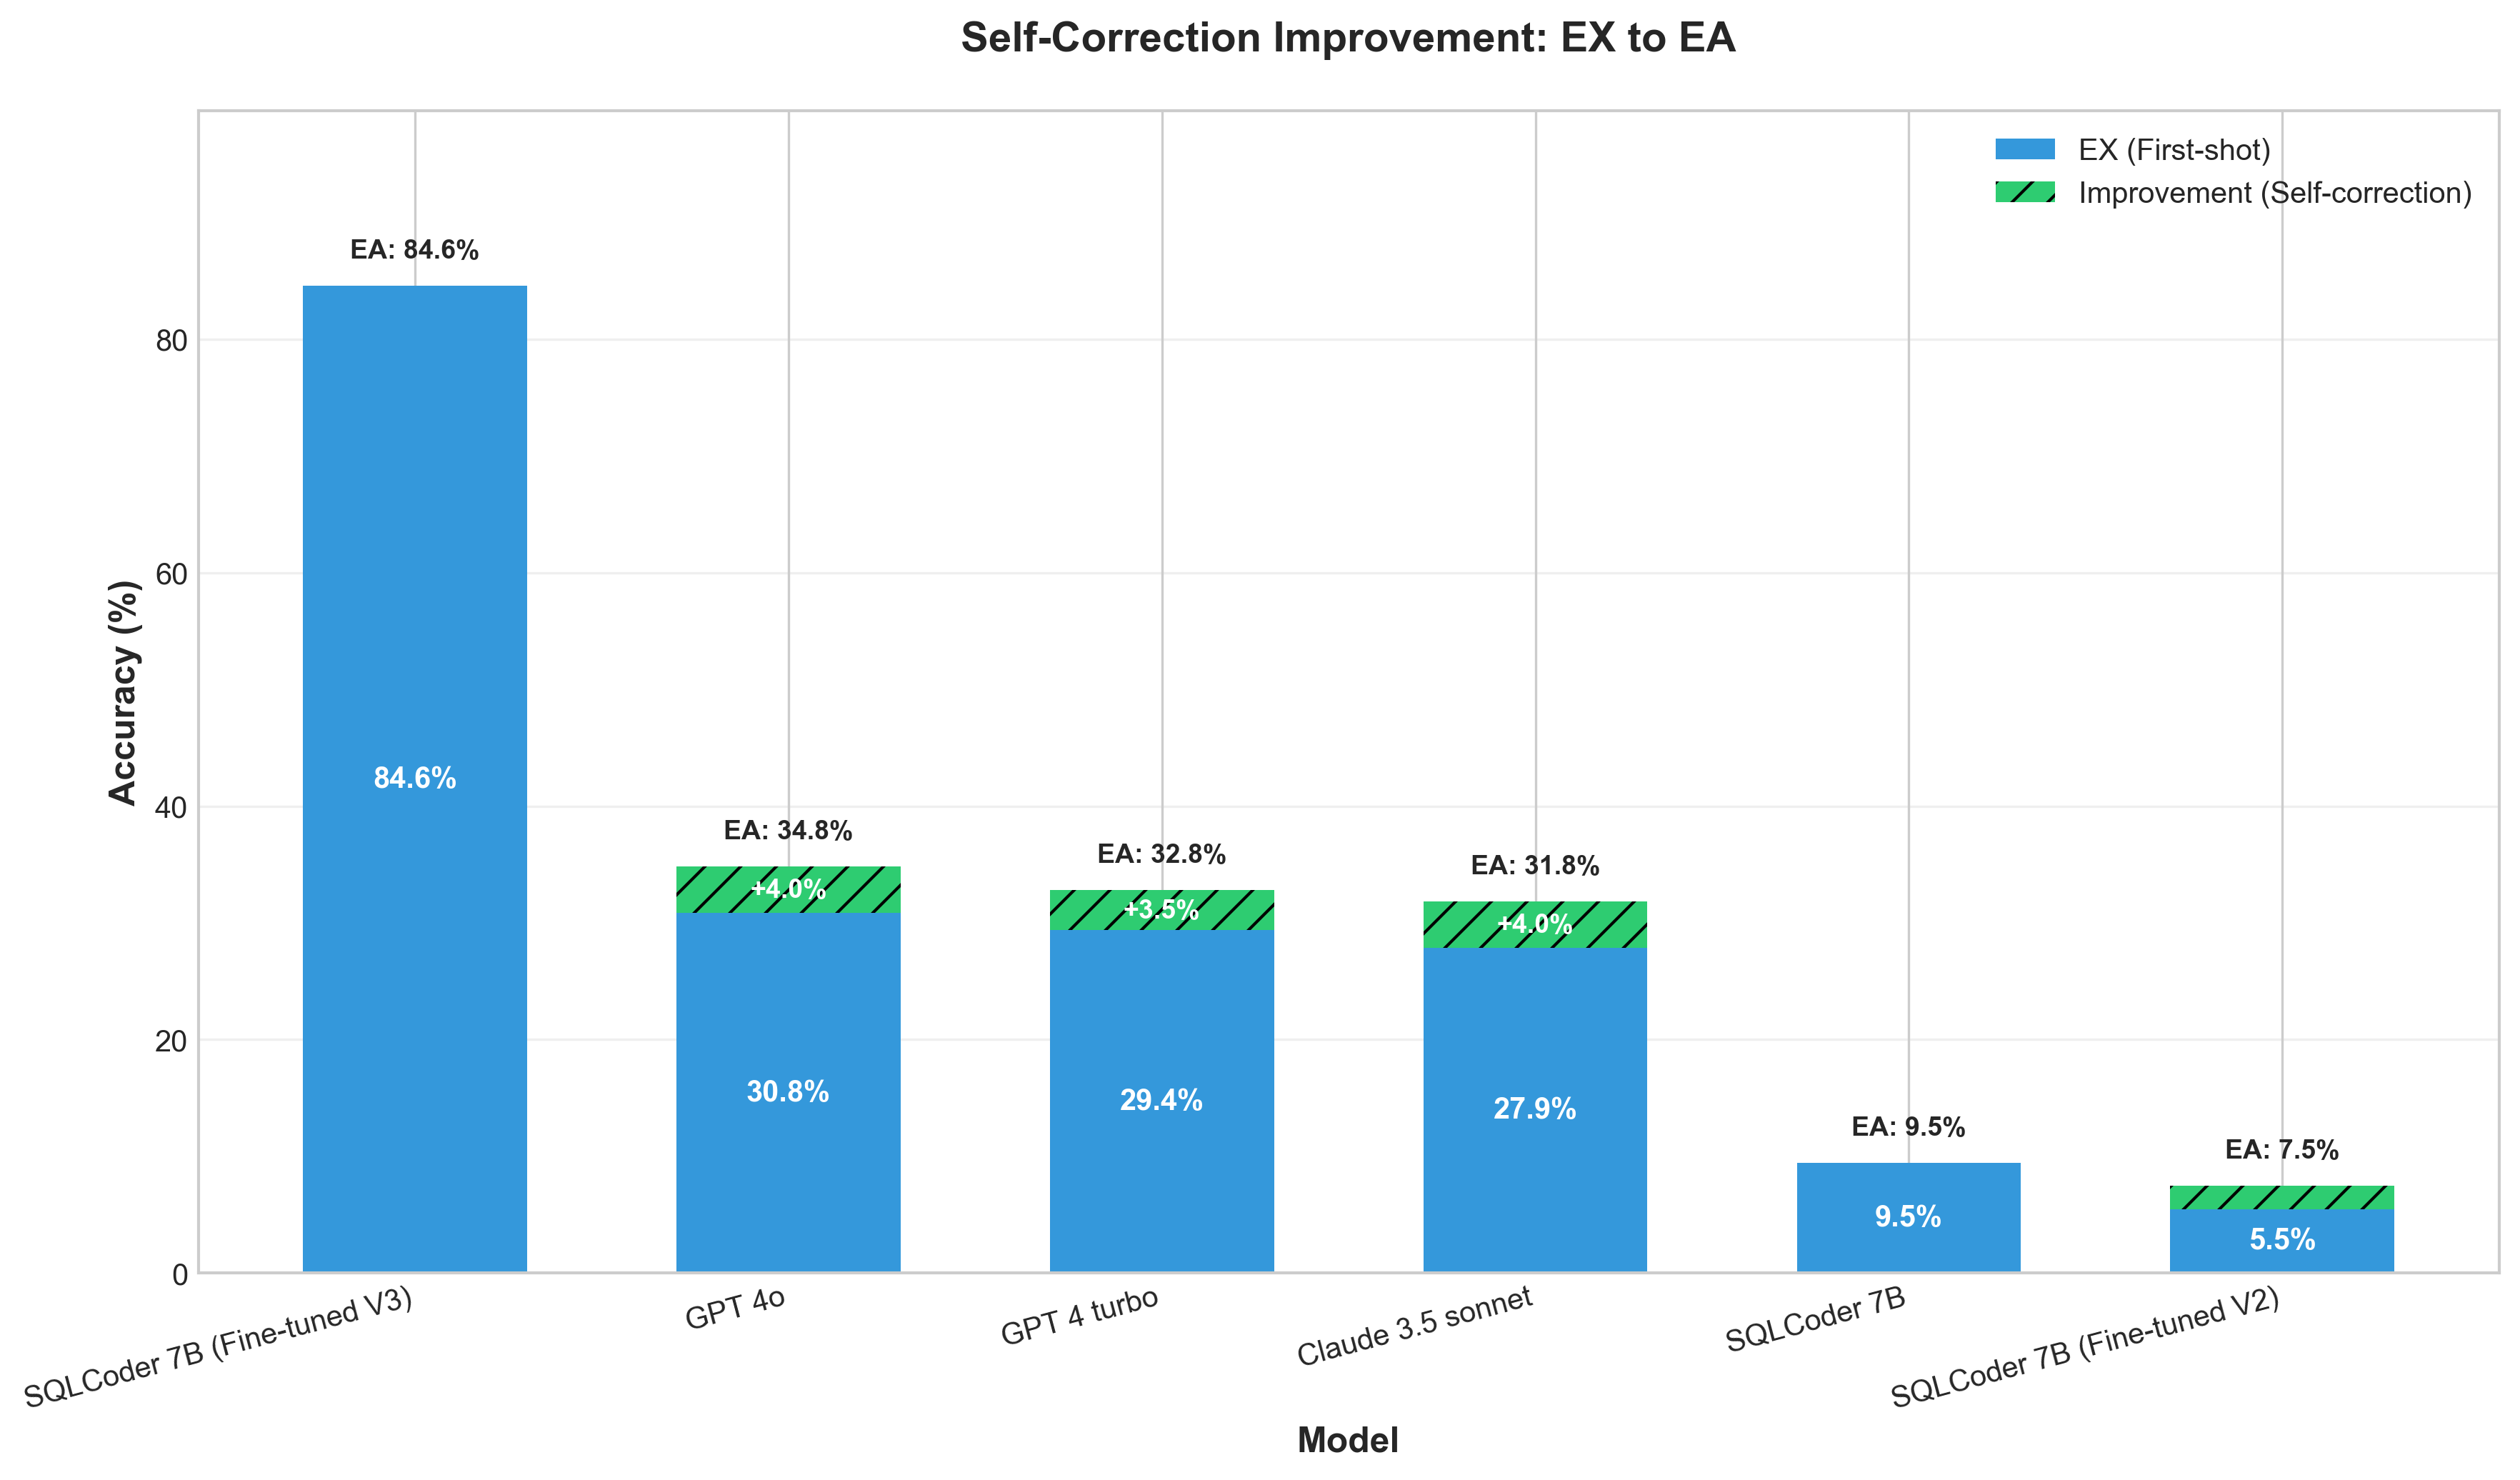
\includegraphics[width=0.95\textwidth,height=0.55\textheight,keepaspectratio]{figures/self_correction.png}
\end{column}
\begin{column}{0.45\textwidth}
\textbf{Key Finding:}\\
\Large SQLCoder EA = EX = \textbf{84.58\%} \normalsize

\vspace{0.3cm}
\textbf{Interpretation:}
\begin{itemize}
    \item Minimal self-correction needed
    \item \textbf{89\% succeed on first attempt}
    \item Average iterations: 1.11
    \item \textcolor{sintefgreen}{High first-shot quality}
\end{itemize}

\vspace{0.3cm}
\begin{block}{Implication}
\textbf{Quality training data > iterative refinement mechanisms}
\end{block}
\end{column}
\end{columns}
\end{frame}

\begin{frame}{Cost-Effectiveness Summary}
\centering
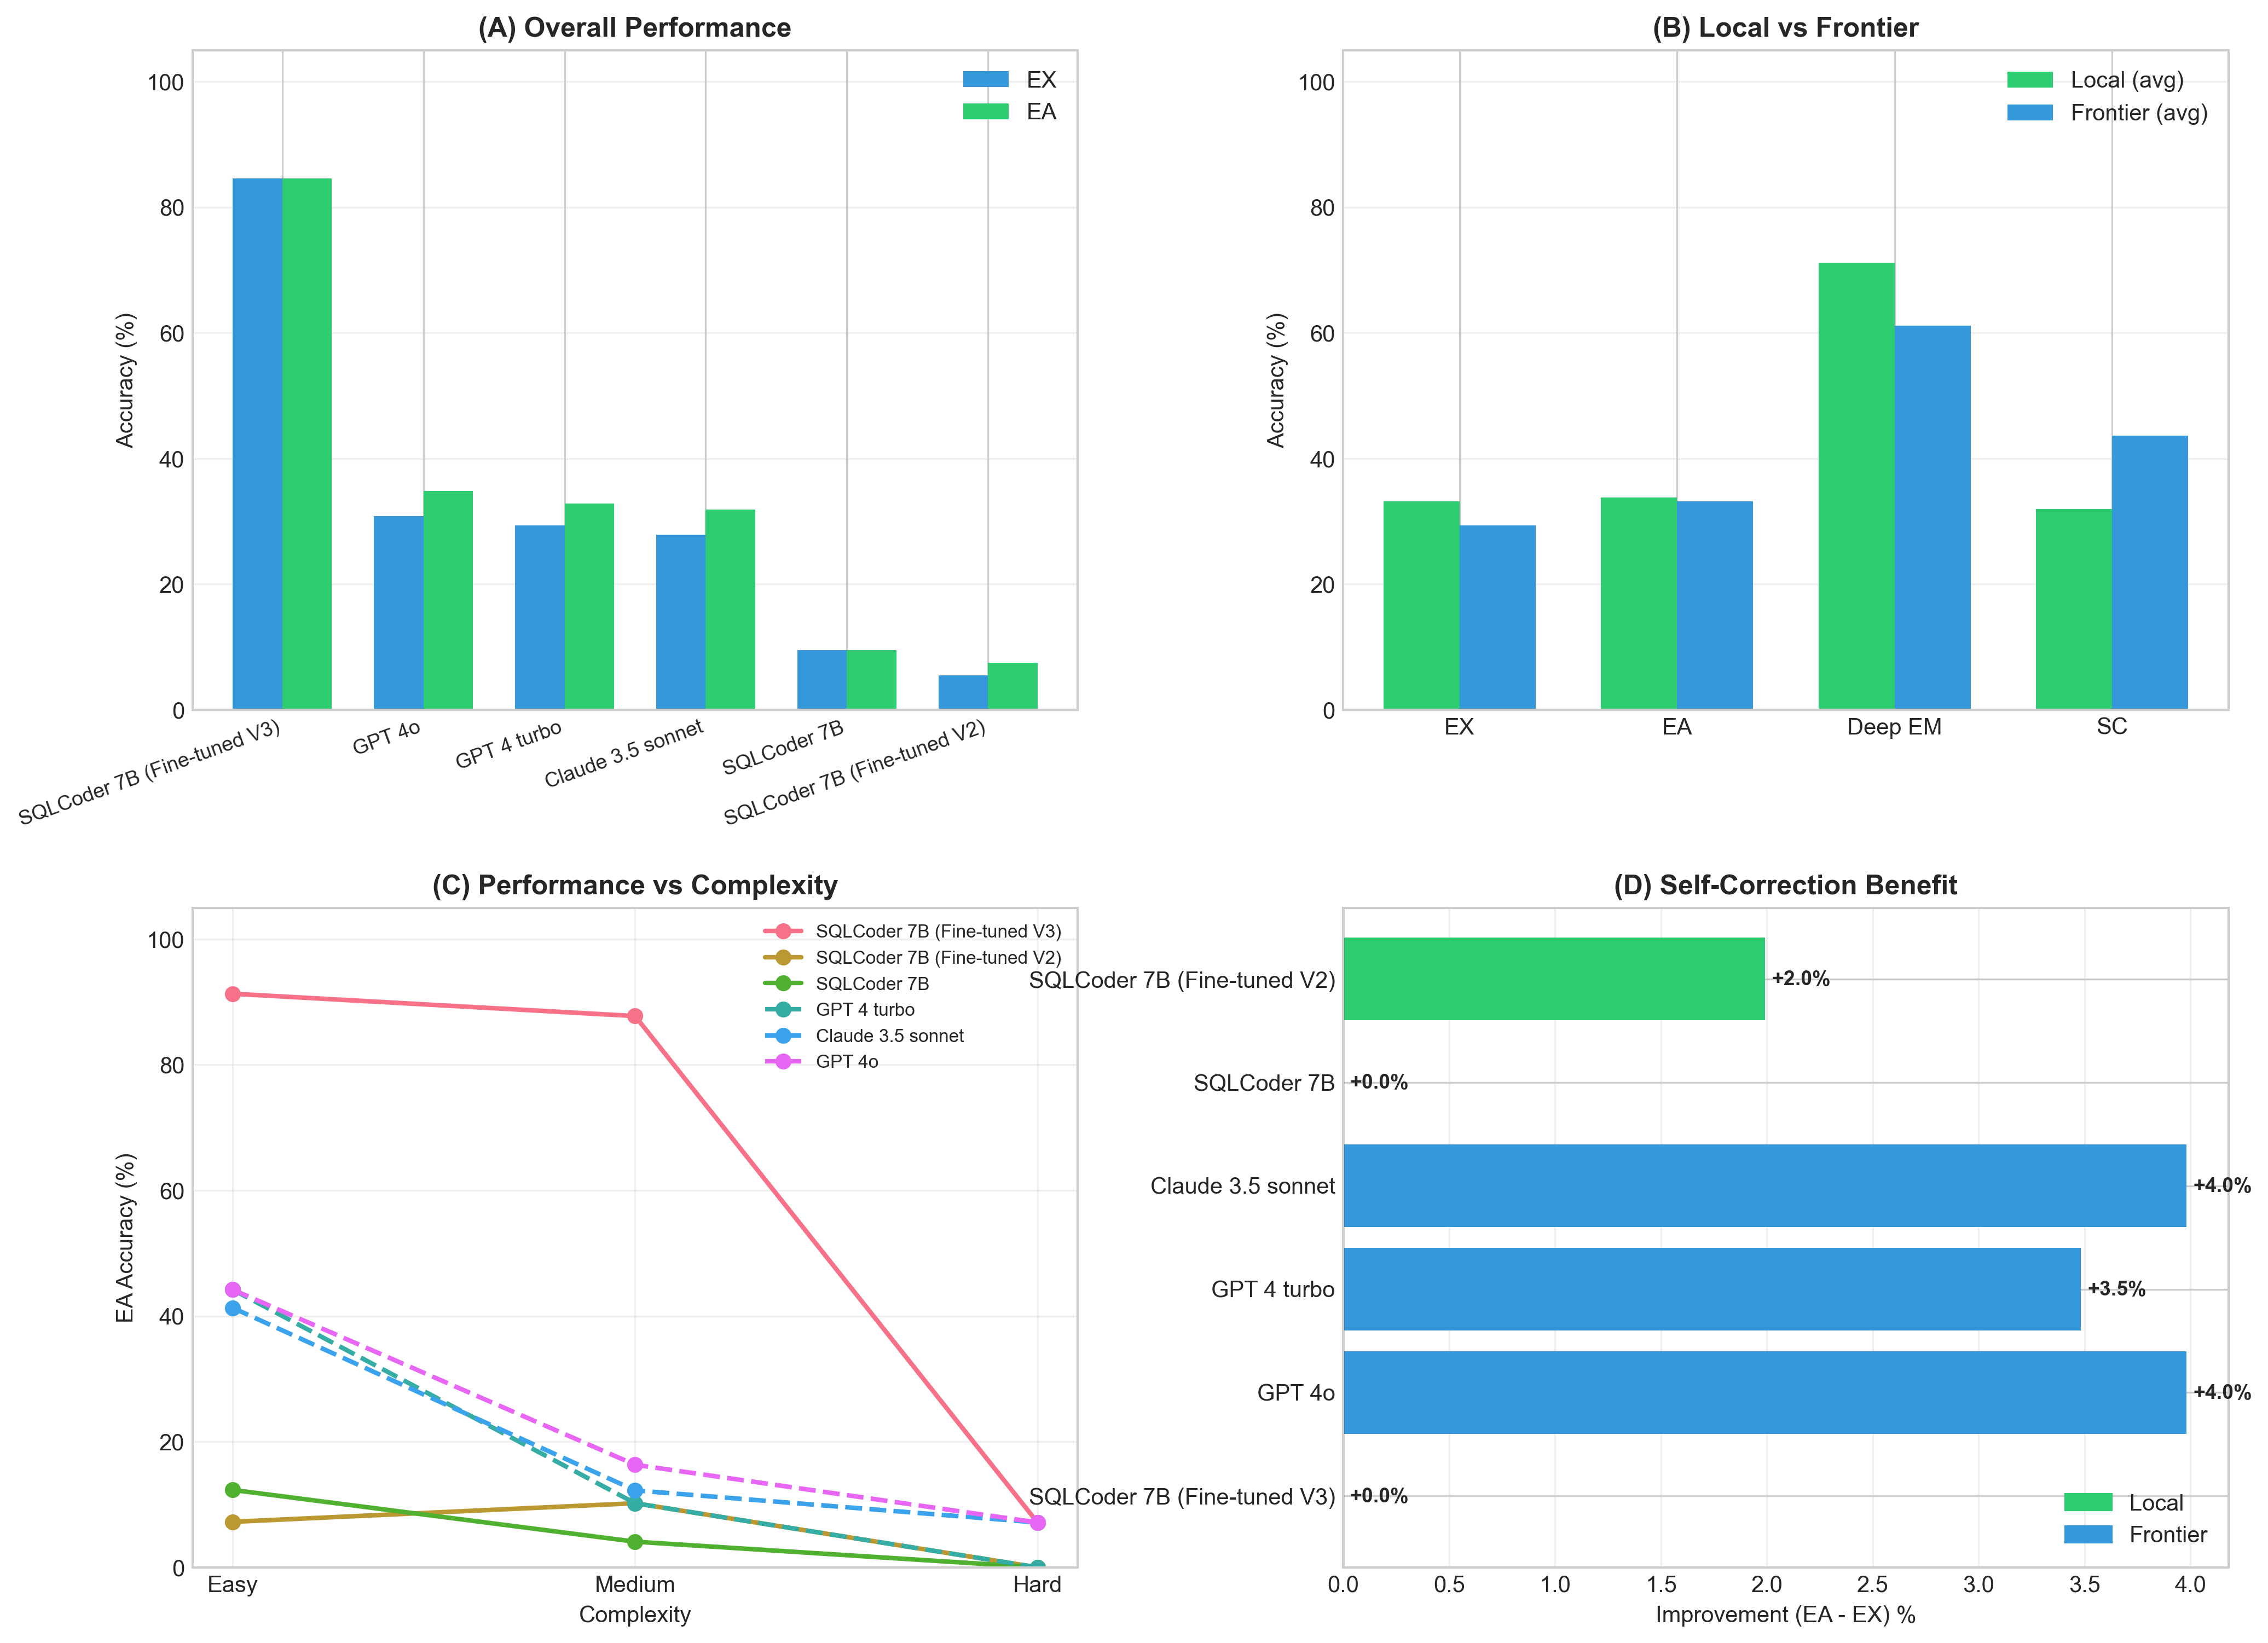
\includegraphics[width=0.85\textwidth,height=0.45\textheight,keepaspectratio]{figures/publication_summary.png}

\vspace{0.2cm}
\begin{columns}
\begin{column}{0.5\textwidth}
\textbf{Dataset Generation:}
\begin{center}
\begin{tabular}{lr}
\toprule
Total Samples & 50,000 \\
NoErr Rate & 97.34\% \\
\textbf{Total Cost} & \textbf{\$50} \\
\bottomrule
\end{tabular}
\end{center}
\textbf{vs Human: \$90,000+}\\
$\rightarrow$ \textcolor{sintefgreen}{\textbf{1,800x savings}}
\end{column}
\begin{column}{0.5\textwidth}
\textbf{Fine-Tuning:}
\begin{center}
\begin{tabular}{lr}
\toprule
Training Time & 51 hours \\
GPU Memory & 18 GB \\
\textbf{Academic Cost} & \textbf{\$0} \\
\bottomrule
\end{tabular}
\end{center}
\textbf{Environmental Impact:}\\
123.5 kWh $\rightarrow$ 34.6 kg CO$_2$\\
($\approx$140 km driving)
\end{column}
\end{columns}
\end{frame}

%=============================================================================
% CONCLUSION (~1 min, 2 slides)
%=============================================================================

\section{Conclusion}

\begin{frame}{Key Contributions \& Insights}
\begin{columns}
\begin{column}{0.5\textwidth}
\textbf{Contributions:}
\begin{enumerate}
    \item \textbf{CIM Wizard Platform}\\
    {\small Calculator-based, multi-schema PostGIS}
    
    \item \textbf{Cost-Effective Dataset}\\
    {\small 50,000 samples at \$50}
    
    \item \textbf{Production-Ready Model}\\
    {\small 84.58\% EX (+54pp over GPT-4o)}
    
    \item \textbf{Evaluation Framework}\\
    {\small 7 metrics, taxonomy-based}
    
    \item \textbf{Open-Source Release}\\
    {\small HuggingFace: taherdoust/ai4cimdb}
\end{enumerate}
\end{column}
\begin{column}{0.5\textwidth}
\textbf{Technical Insights:}
\begin{itemize}
    \item \textbf{Specialization > Scale}\\
    7B fine-tuned beats 100B+ general
    
    \item \textbf{Validation-First Works}\\
    71.5\% retention vs 10-30\%
    
    \item \textbf{Pre-training Matters}\\
    SQLCoder (SQL-specific) > Qwen
    
    \item \textbf{First-Shot Quality}\\
    Self-correction: diminishing returns
\end{itemize}

\vspace{0.3cm}
\textbf{Broader Impact:}\\
Democratizes spatial analytics for urban planners, energy consultants, and policymakers
\end{column}
\end{columns}
\end{frame}

\begin{frame}{Thank You}
\centering
\vspace{1cm}
{\Large \textbf{Questions?}}

\vspace{1cm}
\textbf{Open-Source Resources:}\\
\vspace{0.3cm}
Dataset: \texttt{huggingface.co/datasets/taherdoust/ai4cimdb}\\
\vspace{0.2cm}
Framework: 10,871 lines of code (Apache 2.0)

\vspace{1cm}
\textbf{Future Directions:}\\
{\small CityGML/3DCityDB integration • TimescaleDB temporal data • Multi-lingual support • Cross-domain transfer}

\vspace{1cm}
{\small Ali Taherdoustmohammadi • s299605 • Politecnico di Torino}
\end{frame}

\backmatter

\end{document}
